%\documentclass{sig-alternate-sigmod08}
\documentclass[10pt,conference]{IEEEtran} 
\usepackage{graphicx}
\usepackage{epsfig}
\usepackage{amssymb}
\usepackage{amsfonts}
\usepackage{verbatim}
\usepackage{moreverb}
\usepackage{cancel}
\usepackage{fancyhdr}
\usepackage{algorithmic}
\usepackage{algorithm}
\usepackage{epstopdf}
\usepackage{amssymb,amsfonts,amsmath,amsthm}
\usepackage{subfigure}


%%%%%%%%%%  NEEDS to be commente out to have the nice headers %%%%%
%\pagestyle{fancy}
\DeclareGraphicsRule{.tic}{png}{.png}{`convert #1 `dirname #1`/`basename #1 .tif`.png}

%\textwidth = 6.5 in
%\textheight = 9 in
%\oddsidemargin = 0.0 in
%\evensidemargin = 0.0 in
%\topmargin = 0.0 in
%\headheight = 0.0 in
%\headsep = 0.0 in
%\parskip = 0.2in
%\parindent = 0.0in
%\abovedisplayskip
%\belowdisplayskip
 
%Rnd{\classname}{FOO 699}
\newcommand{\doc}{Technical Report}
\newcommand{\doctitle}{Efficient Recovery from False State in Distributed Routing Algorithms}
\newcommand{\myname}{Daniel Gyllstrom}
%\newcommand{\qed}{\hfill $\Box$ \hfill \\}


\newtheorem{theorem}{Theorem}
\setcounter{theorem}{0}
\newtheorem{claim}[theorem]{Claim}
\newtheorem{conjecture}[theorem]{Conjecture}
\newtheorem{corollary}[theorem]{Corollary}
\newtheorem{fact}[theorem]{Fact}
\newtheorem{lemma}[theorem]{Lemma}
\newtheorem{meta-proposition}[theorem]{Meta-Proposition}
\newtheorem{note}[theorem]{Note}
\newtheorem{observation}[theorem]{Observation}
\newtheorem{proposition}[theorem]{Proposition}
\newtheorem{proviso}[theorem]{Proviso}         
\newtheorem{question}[theorem]{Question}         
\newtheorem{remark}[theorem]{Remark}         
\newtheorem{define}{Definition}     

%\newtheorem{simulation}{Simulation}
\newcounter{simulationCnt}

\newcommand{\simulation}[1]{%
    \stepcounter{simulationCnt}
    \subsubsection{Simulation \arabic{simulationCnt} - }%
 }

%\newcounter{simulation}{0}


\newcommand{\minv}{$\overrightarrow{min}$ }
\newcommand{\minvi}{$\overrightarrow{min}_i$ }
\newcommand{\minvis}{$\overrightarrow{min}_i$}
\newcommand{\minvj}{$\overrightarrow{min}_j$ }
\newcommand{\minvjs}{$\overrightarrow{min}_j$}
\newcommand{\minvv}{$\overrightarrow{min}_v$ }
\newcommand{\minvvs}{$\overrightarrow{min}_v$}
\newcommand{\dmatrix}{$dmatrix$ }
\newcommand{\dmatrixs}{$dmatrix$}
\newcommand{\dmatrixi}{$dmatrix_i$ }
\newcommand{\dmatrixis}{$dmatrix_i$} 
\newcommand{\dmatrixj}{$dmatrix_j$ }
\newcommand{\dmatrixjs}{$dmatrix_j$} 
\newcommand{\dmatrixv}{$dmatrix_v$ }
\newcommand{\dmatrixvs}{$dmatrix_v$} 
%\newcommand{\dmatrixvs}{{\tt dmatrix$_v$}}
\newcommand{\dv}{{DV$^+$ }}
%\newcommand{\bad}{{$\hat{v}$ }}
\newcommand{\Bad}{{$\overline{V}$ }}
\newcommand{\Bads}{{$\overline{V}$}}
\newcommand{\bad}{{$\overline{v}$ }}
\newcommand{\bads}{{$\overline{v}$}}
\newcommand{\alg}{{DV$^+$ }}
\newcommand{\block}{{\tt todo-rename }}
\newcommand{\second}{{{\tt 2}$^{{\tt nd}}$ {\tt best} }}
\newcommand{\seconds}{{{\tt 2}$^{{\tt nd}}$ {\tt best}}}
\newcommand{\infinity}{{count-to-$\infty$ }}
\newcommand{\purge}{{{\tt purge} }}
\newcommand{\purges}{{{\tt purge}}}
\newcommand{\resetall}{{{\tt reset-all} }}
\newcommand{\resetalls}{{{\tt reset-all}}}
\newcommand{\resetk}{{{\tt reset-k} }}
\newcommand{\resetks}{{{\tt reset-k}}}
%\newcommand{\badvector}{{$v_{bad-lie}$ }}
%\newcommand{\oldvector}{{$v_{bad-old}$ }}
\newcommand{\badvector}{$\overrightarrow{bad}$ }
\newcommand{\badvectors}{$\overrightarrow{bad}$}
\newcommand{\oldvector}{$\overrightarrow{old}$ }
\newcommand{\oldvectors}{$\overrightarrow{old}$}
\newcommand{\finalvector}{{$v_{final}$ }}
\newcommand{\illigit}{{illegitimate path} }
\newcommand{\illigits}{{illegitimate paths} }
\newcommand{\lcd}{$\Delta_{lc}$ }
\newcommand{\lcds}{$\Delta_{lc}$s }
\newcommand{\cpr}{{\tt cpr} }
\newcommand{\cprs}{{\tt cpr}}
\newcommand{\er}{Erd\"{o}s-R\'enyi }
\newcommand{\ers}{Erd\"{o}s-R\'enyi} 
\newcommand{\reword}{{\it  Comment: reword}. }
\newcommand{\more}{{\it  Comment: more details needed here}. }
\newcommand{\HRule}{\rule{\linewidth}{0.5mm}}

%newcommand{\block}{{\textsc{block-wait} }}


%%%%%%%%%%%%% This adds the header to each page - currently a bit broken so commented out
%\lhead{\myname{}}
%\chead{\myname{}}
%\rhead{\doc{}}
%\lfoot{}
%

\makeatletter
\newcommand{\un}[1]{%
   % \ifmmode \@@underline{#1} \else %
             $\@@underline{\hbox{#1}}$\fi}
\makeatother
\raggedbottom

\begin{document}




\title{\doctitle}


\author{
\IEEEauthorblockN{Daniel Gyllstrom, Sudarshan Vasudevan, Jim Kurose, Gerome Miklau } 
\IEEEauthorblockA{Department of Computer Science \\ 
University of Massachusetts Amherst \\ 
\{dpg, svasu, kurose, miklau\}@cs.umass.edu}} 
%\andI 
%\IEEEauthorblockN{Sudarshan Vasudevan} 
%\IEEEauthorblockA{Department of Computer Science \\ 
%University of Massachusetts Amherst \\ 
%svasu@cs.umass.edu} 
%\and
%\IEEEauthorblockN{James Kurose} 
%\IEEEauthorblockA{Department of Computer Science \\ 
%University of Massachusetts Amherst \\ 
%kurose@cs.umass.edu} }

\maketitle

%\section{Abstract}

\begin{abstract}

Malicious and misconfigured nodes can inject incorrect state into a distributed system, which can then be propagated system-wide as a result of normal network operation. 
Such false state can degrade the performance of a distributed system or render it unusable. For example, in the case of network routing algorithms, false state corresponding
to a node incorrectly declaring a cost of $0$ to all destinations (maliciously or due to misconfiguration) can quickly spread through the network. This causes other nodes to (incorrectly) 
route via the misconfigured node, resulting in suboptimal routing and network congestion. We propose three algorithms for efficient recovery in such scenarios, prove the correctness 
of each of these algorithms, and derive communication complexity bounds for each algorithm. Through simulation, we evaluate our algorithms -- in terms of message and time overhead -- when 
applied to removing false state in distance vector routing. Our analysis
shows that over topologies where link costs remain fixed and for the same topologies where link costs change, a recovery algorithm based on system-wide checkpoints and a rollback mechanism 
yields superior performance when using the poison reverse optimization.

\end{abstract}
%We propose algorithms that allow distributed routing algorithms to efficiently recover from false state injected into the network.
%We prove the correctness of each algorithm and evaluate them when applied to distance vector routing. In this context, we evaluate the message and time complexity of each algorithm through simulation.

%{\bf Keywords}: {\it distributed algorithms, fault tolerance, routing, security}


\section{Introduction}
\label{sec:intro}

%Distributed systems are vulnerable to malicious and misconfigured nodes which inject false system state. 

Malicious and misconfigured nodes can degrade the performance of a distributed system by injecting incorrect state information. Such false state can then be further propagated 
through the system either directly in its original form or indirectly, e.g., as a result of diffusing computations initially using this false state. 
For example, consider distance vector routing.  If a compromised node incorrectly claims a distance of $0$ to all destinations, this false state would likely
spread throughout the network, infecting shortest paths network-wide.
%For example, with distance vector a compromised node incorrectly claiming a distance of $0$ to all destinations would likely infect shortest paths throughout the network.
In this paper, we consider the problem of removing such false state. % from a distributed system.

In order to make the false-state-removal problem concrete, we investigate distance vector routing as an instance of this problem. Distance vector forms the basis for many routing 
algorithms widely used in the Internet (e.g., BGP, a path-vector algorithm) and in multi-hop wireless networks (e.g., AODV, diffusion routing). However, distance vector is vulnerable 
to compromised nodes that can potentially flood a network with false routing information, resulting in erroneous least cost paths, packet loss, and congestion. Such scenarios have occurred
in practice. For example, in 1997 a significant portion of Internet traffic was routed through a single misconfigured router, rendering a large part of the Internet inoperable for several
hours \cite{Neumann97}. More recently \cite{Google}, a routing error forced Google to redirect its traffic through Asia, causing congestion that left many Google services unreachable. 
Distance vector currently has no mechanism to recover from such scenarios. Instead, human operators are left to manually reconfigure routers. It is in this context that we propose and
evaluate automated solutions for recovery.  We make the following contributions:

\begin{itemize}

\item We design, develop, and evaluate three different approaches -- \seconds, \purges, and \cpr -- for correctly recovering from the injection of false routing state (Section \ref{sec:idea}). 
\second performs localized state invalidation, followed by network-wide recovery using the traditional distance vector algorithm (Section \ref{subsubsec:second}).
The \purge algorithm performs global false state invalidation by using diffusing computations to invalidate distance vector 
entries (network-wide) that routed through a compromised node (Section \ref{subsubsec:purge}). Then, traditional distance vector routing is used to recompute distance vectors.
\cpr uses local snapshots and a rollback mechanism to implement recovery (Section \ref{subsubsec:cpr}). 

\item We prove the correctness of each algorithm for scenarios of single and multiple compromised nodes (Section \ref{sec:correct}). 
A recovery algorithm is correct if the routing tables for all nodes have converged to a global state in which all nodes 
have removed each compromised node as a destination and no node bears a least cost path to any destination that routes through a compromised node.

\item We derive communication complexity bounds for each algorithm over a synchronous communication model (Section \ref{sec:analysis}).  
%In some scenarios, we find the exact number of messages each node sends in order recover. 
We find all three algorithms are bounded above by $O(mnd)$ -- where $d$ is the diamter, $n$ is the number of nodes, and $m$ the maximum out-degree of any node -- in scenarios where 
link costs remain fixed.  In scenarios where link costs can change, \cpr incurs additional overhead (not experieced by \second and \purges) because \cpr must update stale
state after rolling back.  This leads to an additional term for \cpr in its $O(mnd)$ upper bound. %\cpr has an additional term

\item Using simulations, we evaluate the efficiency of each algorithm in terms of message overhead and convergence time in scenarios with single and 
multiple compromised nodes. (Section \ref{sec:eval}).
Our simulations show that \cpr using poison reverse outperforms \second and \purge (with and without poison reverse) -- at the cost of checkpoint memory --
over topologies with fixed and changing link costs. This is because \cpr efficiently removes all false state by rolling back to a checkpoint
immediately preceding the injection of false routing state. 

\item We show through simulations that \purge using poison reverse yields performance close to \cpr with poison reverse in scenarios where link costs can change
(Section \ref{subsec:change}). \purge makes use of computations subsequent to the injection of false routing state that do not depend on false routing state, while \cpr 
must process all valid link cost changes that occurred since false routing state was injected.  Finally, our simulations show that poison reverse significantly improves 
performance for all three algorithms, especially for topologies with changing link costs (Section \ref{subsubsec:pr-fixed} and \ref{subsubsec:pr-change}). % by removing pairwise routing loops.

\end{itemize}

Recovery from false routing state is closely related to the problem of
recovering from malicious transactions \cite{Liu98,Liu00} in
distributed databases. Our problem is also similar to that of rollback
in optimistic parallel simulation \cite{Jeff}. However, we are unaware
of any existing solutions to the problem of recovering from false
routing state. A closely related problem to the one considered in this
paper is that of discovering misconfigured nodes. In
Section~\ref{sec:problem}, we discuss existing solutions to this
problem. In fact, the output of these algorithms serve as input to the
recovery algorithms proposed in this paper.








%%%%%%%%%%%%%%%%%%%%%% IDEAS SECTIOn %%%%%%%%%%%%%%%%%%
\section{Paper Intuition}
%\section{The Idea}
\label{sec:idea}

\subsection{The Problem}
\label{subsec:problem}

We address the problem of recovering from false routing state in distance vector routing.
We assume nodes are compromised such that they declare false routes to all other nodes in the network. 
{\footnote {\small  For simplicity, in this section we present our recovery algorithms in the case of a single compromised node.  The necessary extensions to handle multiple compromised nodes are 
 addressed in our Technical Report \cite{Tech}.}}
This false state spreads through the network through the normal execution of distance vector, leading to erroneous least cost paths.  We assume that the identity of the 
compromised node is provided by a different algorithm \cite{Arini,Feam,Vishal02,Pad03,Paul02}, and thus do not consider this problem in this paper.
Instead, we focus on recovering after receiving notification that a node is compromised.  The goal is for all nodes to recover correctly: each node  should 
remove the compromised node as a destination and find new least cost distances that do not use a compromised node. 
{\footnote {\small If the network becomes disconnected as a result of removing the compromised node, all nodes need only compute new least cost distances to all other nodes 
within their connected component. }}



Consider the example graph, $G$, in Figure \ref{fig:example}. Figure \ref{fig:example-a} shows $G$ before \bad is compromised. 
{\footnote {\small For convenience, we refer to \bad as the generic compromised node in the remainder of the document.}}
At this point, all least costs are correctly computed.
 {\footnote {\small Node $i$ and $j$'s routing table are shown to the right of $G$.  The least costs are underlined.}}
Now, let \bad be compromised such that it falsely declares a cost of $1$ to every other node.  Consistent with ``good news travels fast'', these false paths spread through the network,
leading to erroneous least cost paths.  For example, 
Figure \ref{fig:example-b} depicts the state of $G$ after \bads's false routing state has propagated throughout the network.  
$i$ routes via \bad to reach nodes $l$ and $d$.  $j$ uses $i$ to reach all nodes except $l$, which implies $j$ transitively uses \bad to reach these destinations 
(e.g., $j$ uses the path $j-i-\overline{v}$ then the false path from \bad to the destination). Upon receiving notification that \bad is compromised, the goal of the 
recovery is to reach the state depicted in Figure \ref{fig:example-c}: \bad is removed as a destination and no least cost uses \bad as an intermediate node. 


%Consider the example graph, $G$, in Figure \ref{fig:example}. Figure \ref{fig:example-a} shows $G$ before any nodes are compromised. All least costs are correctly computed and
%parts of node $i$ and $j$'s routing table are shown to the right of $G$.  The least costs are underlined.  Now, let \bad be compromised such that it falsely declares a cost of $1$
%to every other node.  Consistent with ``good news travels fast'', these false paths spread through the network, leading to erroneous least cost paths.  For example, 
%Figure \ref{fig:example-b} depicts the state of $G$ after \bads's false routing state has propagated throughout the network.  
%$i$ routes via \bad to reach nodes $l$ and $d$.  $j$ uses $i$ to reach all nodes except $l$.  Notice that when $j$ uses $i$ to reach $d$, it transitively uses \bad 
%(e.g., uses path $j-i-$\bads$-d$ to $d$). 

%In our problem setting, we assume an outside algorithm \cite{Arini,Feam,Vishal02,Pad03,Paul02} identifies the compromised node: in this case, \bads. From this point, the goal of the 
%recovery is to reach the state depicted in Figure \ref{fig:example-c}: \bad is removed as a destination and no least cost uses \bad as an intermediate node. 


\begin{figure*}[t]
  \begin{center}
    \subfigure[Before \bad is compromised.]{\label{fig:example-a}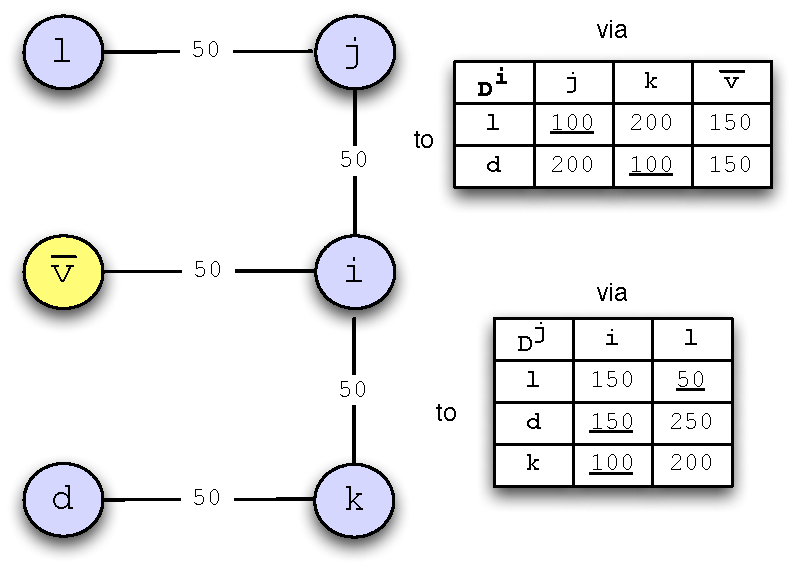
\includegraphics[scale=0.43]{figs/example-a-color.pdf}}
    \subfigure[After \bad is compromised.]{\label{fig:example-b}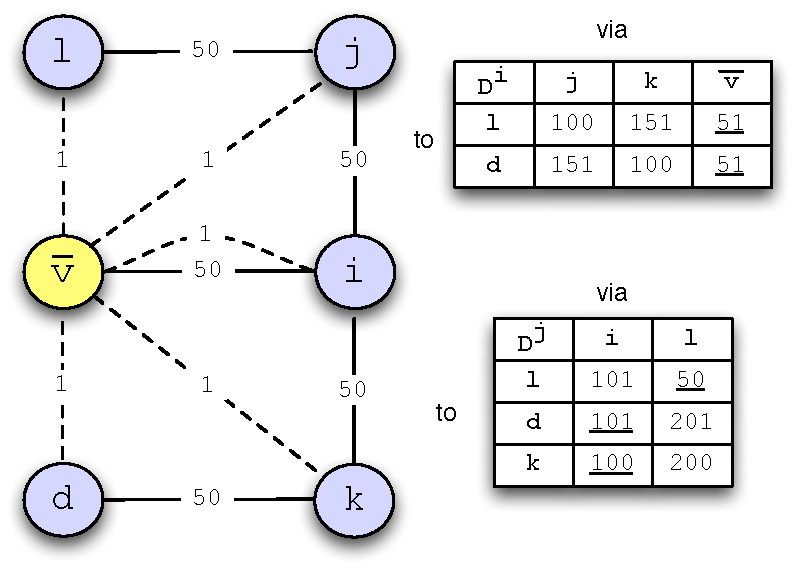
\includegraphics[scale=0.43]{figs/example-b-color.pdf}} 
    \subfigure[After recovery.]{\label{fig:example-c}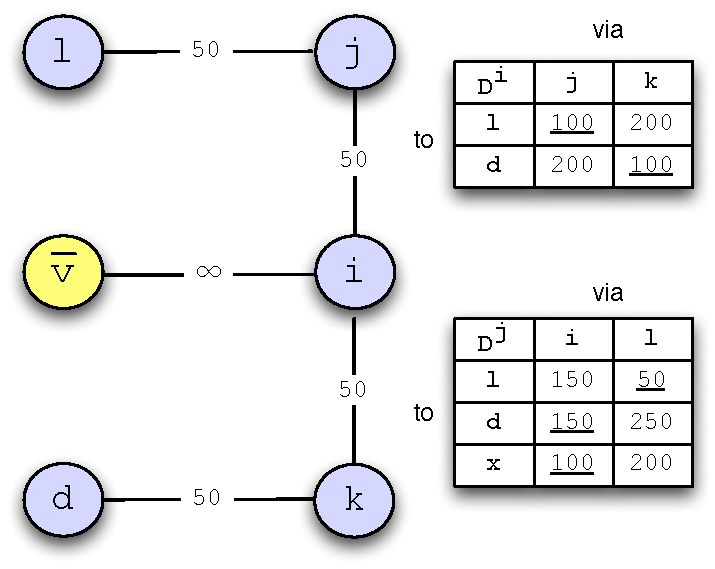
\includegraphics[scale=0.43]{figs/example-c-color.pdf}}
  \end{center}
	\caption{Three snapshots of a graph, $G$, where \bad is the compromised node: (a) $G$ before \bad is compromised, (b) $G$ after false state has 
	finished propagating but before recovery has started, and (c) $G$ after recovery. The dashed lines in (b) mark false paths. Portions of node $i$'s and $j$'s 
	routing table are displayed to the right of each sub-figure. The least cost values are underlined.}
  \label{fig:example}
\end{figure*}


\subsection{Our Solutions}
\label{subsec:algs}

In this section we propose three new recovery algorithms: \seconds, \purges, and \cprs.  The input and output of each algorithm is the same.  The input for each
algorithm is an undirected graph, correctly computed least cost paths to all nodes, and the identity of the compromised node.  The output of each 
algorithm is a new undirected graph with the compromised node removed and new least cost paths that route around the compromised node. 

First we describe a preprocessing procedure common to all three recovery algorithms. Then we describe each recovery algorithm.

\subsubsection{Preprocessing Procedure}
\label{subsubsec:preprocess}
	
All three recovery algorithms share a common preprocessing procedure.  The procedure removes the compromised node as a destination and finds the node IDs in each connected component. 
This is implemented using diffusing computations \cite{Dijkstra80} initiated at each neighbor of the compromised node. A diffusing computation is a distributed algorithm started at a source
node which grows by sending queries along a spanning tree, constructed
simultaneously as the queries propagate through the network.  When the computation reaches the leaves
of the spanning tree, replies travel back along the tree towards the
source, causing the tree to shrink. The computation eventually terminates when the
source receives replies from each of its children in the tree. 

Consider the example in Figure \ref{fig:example} where \bad is the compromised node. 
When $i$ receives the notification that \bad has been compromised, $i$ removes \bad as a destination and then initiates a diffusing computation. 
$i$ creates a vector and adds its node ID to the vector. $i$ sends a message containing this vector to $j$ and $k$.  Upon receiving $i$'s message,
$j$ and $k$ both remove \bad as a destination and add their own ID to the message's vector.  Finally, $l$ and $d$ receive a message from $j$ and $k$, respectively.  
$l$ and $d$ add their own node ID to the message's vector and remove \bad as a destination. Then, $l$ and $d$ send an ACK message back to $j$ and $k$, respectively, with the complete 
list of node IDs. Eventually when $i$ receives the ACKs from $j$ and $k$, $i$ has a complete list of nodes in its connected component. Finally, $i$ broadcasts the vector of node IDs
in its connected component. 

\subsubsection{The 2$^{nd}$ Best Algorithm}
\label{subsubsec:second}


\second invalidates state locally and then uses distance vector to implement network-wide recovery.  Following the preprocessing described in Section \ref{subsubsec:preprocess}, 
each neighbor of the compromised node locally invalidates state by selecting the least cost pre-existing path that does not use the compromised node as the first hop.
The resulting distance vectors trigger the execution of traditional distance vector, which removes the remaining false state.

We trace the execution of \second using the example in Figure \ref{fig:example}.
%In Figure \ref{fig:example-b}, $i$ uses \bad to reach nodes $l$ and $d$.  $j$ uses $i$ to reach all nodes except $l$.  Notice that when $j$ uses $i$ to reach $d$, 
%it transitively uses \badvector (e.g., uses path $j-i-$\bads$-d$ to $d$). 
After the preprocessing completes, $i$ selects a new neighbor to route through to reach $l$ and $d$ by finding its new smallest distance in its local routing table
to these destinations: $i$ selects the routes via $j$ to $l$ with a cost of $100$ and $i$ picks the route via $k$ to reach $d$ with cost of $100$. 
(No changes are required to route to $j$ and $k$ because $i$ uses its direct link to these two nodes). 
Then, $i$ sends its new least cost vector to its neighbors, triggering the execution of traditional distance vector.


\subsubsection{The purge Algorithm}
\label{subsubsec:purge}


\purge globally invalidates all false state using a diffusing computation and then uses distance vector to compute new distance values that avoid all invalidated paths.
{\footnote {\small Because diffusing computations preserve the decentralized nature of distance vector, \purge is a decentralized algorithm.}}
The diffusing computation is initiated at the neighbors of the compromised node (\bads) because only these nodes are 
aware if \bad is used an intermediary node along a given path. The diffusing computations spread from \bads's neighbors to the network edge, invalidating false state at each node along the way. 
Then ACKs travel back from the network edge to the neighbors of \bads, indicating that the diffusing computation is complete. 
%See Algorithm \ref{alg:purge} and \ref{alg:purge2} in the Appendix for a complete specification of this diffusing computation.
Finally, \purge uses distance vector to recompute least cost paths invalidated by the diffusing computations.  

In Figure \ref{fig:example}, the diffusing computation executes as follows. First, $i$ sets its distance to $l$ and $d$ to $\infty$ (thereby invalidating $i$'s path to $l$ and $d$)
because $i$ uses \bad to route these nodes. Then, $i$ sends a message to $j$ and $k$ containing $l$ and $d$ as invalidated destinations.
When $j$ receives $i$'s message, $j$ checks if it routes via $i$ to reach $l$ or $d$. Because $j$ uses $i$ to reach $d$, $j$ sets its distance estimate to $d$ to $\infty$. 
$j$ does not modify its least cost to $l$ because $j$ does not route via $i$ to reach $l$. Next, $j$ sends a message that includes $d$ as an invalidated destination.
$l$ performs the same steps as $j$. After this point, the diffusing computation ACKs travel back towards $i$. When $i$ receives an ACK, the diffusing computation is complete. At this
point, $i$ needs to compute new least costs to node $l$ and $d$ because $i$'s distance estimates to these destinations are $\infty$. To do so, $i$ uses its local routing table to find 
its new least cost to $l$ and $d$. This triggers the execution of distance vector, which recomputes least cost paths invalidated by the diffusing computations.

\purge is very similar to Garcia-Lunes-Aceves's DUAL algorithm \cite{JJ93}. 
{\footnote {\small \purge was designed prior to the authors' efforts to consider the DUAL algorithm as a solution to the false-state recovery problem.}} 
%The DUAL algorithm was designed to ensure loop-free routing in cases of link and node failure.  
DUAL uses diffusing computations to coordinate least cost computations after a node (or link) fails. 
{\footnote {\small {Although DUAL does not explicitly consider the false routing state problem, with some minor changes DUAL can be adapted to recover in such scenarios. 
DUAL assumes nodes locally detect a failing node.  In contrast, our algorithms assume detection is handled by an outside algorithm.  Thus, DUAL must be modified such that all nodes accept input from a detection algorithm. }}
The diffusing computations find a next-hop node -- called a feasible successor --  which ensures loop freedom.  Once a node 
finds a feasible successor and has received replies (corresponding to a diffusing computation) from all child nodes, the node operates according to distance vector:
if a new least cost is selected, an update is sent to the node's neighbors. 
{\footnote {\small DUAL does not explicitly invalidate routing state from a failed node but DUAL's diffusing computations to find a feasible successor have a similar effect. }}
As with \purges, this ensures that only valid paths are shared.  


%{\footnote {\small DUAL does not explicitly consider the false routing state problem but with some minor changes it can be adapted to recover in such scenarios. 
%Specically, DUAL assumes nodes locally detect a failing node.  We however assume detection is handled by an outside algorithm.  As such, nodes running DUAL must be able to accept
%input from a detection algorithm. }} 
%DUAL does not explicitly invalidate routing state from a failed node but DUAL's diffusing computations to find a feasible successor have a similar effect. 
%A feasible successor is a next-hop node (along a shortest path) which cannot cause a routing loop.  DUAL ensures a loop-free successor is selected by using 
%diffusing computations to coordinate least cost computations after a node fails.  Once a node 
%finds a feasible successor and has received replies from all child nodes, the node operates according to distance vector: if a new least cost is selected, an update is sent to the node's 
%neighbors.  As with \purges, this ensures that only valid paths are shared.  

A subtle difference between DUAL and \purge is that \purge initiates distance vector computations -- to recompute valid paths to destinations invalidated by the diffusing computations --
from the neighbors of the compromised node, while DUAL starts distance vector computations once a node finds a feasible successor and has received replies from all child nodes. 
With DUAL, this occurs close to the leaves of the diffusing computation spanning trees. % Otherwise, \purge and DUAL are identical. We compare the two algroithms in our simulation study \ref{sec:eval}.
%Because this is the only difference between \purge and DUAL, we are able to compare these design decisions in our simulation study \ref{sec:eval}.

%Our simulation results show that initiating diffusing computations closer to the failed node is more efficient (as evidenced by the slightly improved performance of \purge over DUAL).

{\bf todo may want to mention purge is loop free?}



\subsubsection{The cpr Algorithm}
\label{subsubsec:cpr}

\cpr adds a time dimension to each node's routing table, which \cpr  uses to locally archive a complete history of values.  The routing table snapshots are taken either at a given 
frequency or after some number of distance value changes (e.g., each time a distance value changes). Once nodes are notified that a node is compromised, the nodes roll back to a 
snapshot taken before \bad was compromised. Then, \cpr removes \bad as destination and runs distance vector to update stale distance values resulting from link cost changes.

In the example from Figure \ref{fig:example}, \cpr has a snapshot that reflects the system state shown in Figure \ref{fig:example-a}.  After \bad is compromised, \cpr rolls back 
to said snapshot.  Finally, \cpr runs standard distance vector to update the stale state (e.g., $(i,$\bads$)=50$ in the snapshot rather than $\infty$).





%%%%%%%%%%%%%%% For synthesis report - Defines problem statement %%%%%%%%%
\section{Formal Problem Statement and Notation}
\label{sec:problem}

We consider distance vector routing \cite{Gall87,Ford62} over arbitrary network topologies. We model a network as an undirected graph, $G=(V,E)$,
with a link weight function $w: E \rightarrow \mathbb{N}$.
{\footnote {\small Recovery is simple with link state routing: each node uses its complete topology map to compute new least cost paths that avoid all compromised nodes.
Thus we do not consider link state routing in this paper.}}
Each node, $v$, maintains the following state as part of distance vector: a vector of all adjacent nodes ($adj(v)$), a vector of least cost distances to all
nodes in $G$ (\minvvs), and a \emph{distance matrix} that contains distances to every node in the network via each adjacent node (\dmatrixvs). 

We make the following assumptions about the distance vector computation. All initial \dmatrix values are non-negative. Furthermore, all \minv values periodically
exchanged between neighboring nodes are non-negative. All $v \in V$ know their adjacent link costs. All link weights in $G$ are non-negative and do not change.
$G$ is finite and connected. Finally, we assume reliable communication. 

We assume that the identity of the compromised nodes -- which we refer to as $\overline{V}$ -- are provided by a different algorithm \cite{Arini,Feam,Vishal02,Pad03,Paul02}.
Specifically, we assume that at time $t_b$, this algorithm detects all compromised nodes and notifies the neighbors of each compromised node.  Let $t'$ be the time the first node was compromised.

For each algorithm, the goal is for all nodes to recover correctly: all nodes should remove all compromised nodes as a destination and find
new least cost distances that do not use a compromised node. If the network becomes disconnected as a result of removing the compromised nodes, all
nodes need only compute new least cost distances to all other nodes within their connected component.  With one exception, the input and output of each algorithm is the same. 
{\footnote {\small Additionally, as input \cpr requires that each $v \in adj($\bads$)$ is notified of the time, $t'$, in which \bad was compromised.}}
\begin{itemize}

	\item {\bf Input:}  Undirected graph, $G=(V,E)$, with weight function $w: E \rightarrow \mathbb{N}$.  $\forall v \in V$,  \minvv and \dmatrixv are computed
	(using distance vector). Also, each $v \in adj($\bads$)$ is notified that \bad was compromised.

	\item {\bf Output:} $G'=(V',E')$, where $V' = V - \overline{V}$, $E'=E - \{(\overline{v},v_i)$ $|$ $\overline{v} \in \overline{V} \wedge v_i \in adj(\overline{v}) \}$.
	%Undirected graph, $G'=(V',E')$, where $V' = V -\{$\bads$\}$, $E'=E - \{(\bar{v},v_i)$ $|$ $v_i \in adj(\bar{v}) \}$,
\end{itemize}
For convenience, $|V| = n$ and the diameter of $G'$ is $d$. Let $\displaystyle \max_{i \in V'}(|adj(i)|) = m$.  

For an arbitrary $\overline{v} \in \overline{V}$ we use the following notation. \oldvector refer to $\overrightarrow{min}_{\overline{v}}$ before \bad was compromised.
\badvector denotes $\overrightarrow{min}_{\overline{v}}$ after \bad has been compromised.
Intuitively, \oldvector and \badvector are snapshots of the compromised node's least cost vector taken at two different timesteps: \oldvector marks the snapshot taken before \bad was compromised and 
\badvector represents a snapshot taken after \bad was compromised.

Let $\delta_t(i,j)$ be the least cost between nodes $i$ and $j$ -- used by node $i$ --  at time $t$ (we refer to this cost as $\delta(i,j)$).
$p_t(i,j)$ refers to $i$'s actual least cost path to $j$ at time $t$.
 $p_s(i,j)$ is the least cost path from node $i$ to $j$ used by $i$ at $t_b$
and $\delta_s(i,j)$ is the cost of this path; $p_u(i,j)$ is $i$'s least cost path to $j$ at time $t \in [t_b,t^*]$ and $\delta_u(i,j)$ the cost of this path 
{\footnote {\small $p_u(i,j)$ and $\delta_u(i,j)$ can change during $[t_b,t^*]$.}}; and $p_f(i,j)$ is $i$'s final least cost path to $j$ (least cost at $t^*$)
 and has cost $\delta_f(i,j)$.  $\ell(i,j)$ is the minimum number of links between nodes $i$ and $j$ in $G'$.  


For each algorithm, let $t^*$ mark the time when the recovery algorithm completes. Let $\hat{t}$ be the time all diffusing computations complete.  Recall with \purges, \bad is removed as a destination and 
\badvector state is invalidated in the \emph{same} diffusing computations.   Likewise, each \cpr diffusing computation performs two actions: 
the diffusing computations remove \bad as a destination \emph{and} implement the rollback.  For this reason, $\hat{t}$ marks the same time across all three recovery algorithms. 
Let $C(i,j) = \delta_f(i,j) - \delta_{\hat{t}}(i,j)$.  That is, $C(i,j)$ refers to the magnitude of change in $\delta(i,j)$ after the diffusing computations for each algorithm complete.

Table \ref{tab:abbrev} summarizes the notation used in this document and all important timesteps are shown in Figure \ref{fig:timeline}.

\begin{table}[t]
\begin{center}
\begin{tabular}{l l} 
\hline \hline
   	{\bf Notation} & {\bf Meaning} \\
		  \hline 
			$\overline{V}$ & set of compromised nodes \\ 
		  	$G$ &  undirected graph $(V,E)$, with weight function $w: E \rightarrow \mathbb{N}$ \\
			$G'$ & undirected graph $(V',E')$, where $V' = V - \overline{V}$,  \\
			 & $E'=E - \{(\overline{v},v_i)$ $|$ $\overline{v} \in \overline{V} \wedge v_i \in adj(\overline{v}) \}$ \\
			$adj(v)$ & nodes adjacent to $v$ in $G'$ \\ 
 		 	$n$ & $|V|$ \\
			$d$ & diameter of $G'$  \\
			$m$ & $\displaystyle \max_{i \in V'}(|adj(i)|) = m$  \\
 			$\ell(i,j)$ & minimum number of links between nodes $i$ and $j$ in $G'$ \\
			\dmatrixi & node $i$' distance matrix \\
			\minvi & node $i$'s the least cost vector \\
			\badvector & compromised node's least cost vector at $t \geq t'$ \\ %and after $t$  \\
			\oldvector & compromised node's least cost vector at $t < t'$ \\ %and before $t'$ \\
			\hline
			$p_t(i,j)$ & $i$'s actual least cost path to $j$ at time $t$. \\
			$\delta_t(i,j)$ & $i$'s least cost between nodes to $j$ at time $t$ \\
			$p_s(i,j)$ & $i$'s least cost path to $j$ at time $t_b$ \\
			$\delta_s(i,j)$ & $i$'s least cost to $j$ at time $t_b$ \\
			$p_u(i,j)$ & $i$'s least cost path to $j$ at time $t \in [t_b,t^*]$ \\
			$\delta_u(i,j)$ & $i$'s least cost to $j$ at time $t \in [t_b,t^*]$ \\
			$p_f(i,j)$ &  $i$'s least cost path to $j$ at $t^*$ \\
			$\delta_f(i,j)$ &  $i$'s least cost to $j$ at $t^*$ \\
			\hline
			$t_b$ & time the compromised node is detected \\
			$t'$ & time the compromised node was compromised \\
			$t^*$ & time when recovery algorithm completes \\
			$\hat{t}$ & time all diffusing computations complete \\
			\hline \hline
			\end{tabular}
			\end{center}
\caption{Notation Table}
			%* The distance matrix for node $v$ contains $v$'s distance to all nodes $v_d \in V$ via all $v_n: v_n \in adj(v)$.}
\label{tab:abbrev}
\end{table}



\begin{figure}
\begin{center}
\begin{picture}(200,55)
\put(0,25){\vector(1,0){220}}  % pi and to the right
\put(0,25){\vector(-1,0){20}}  % pi and to the right

%tics
\put(20,22){\line(0,1){6}} 
\put(70,22){\line(0,1){6}} 
\put(120,22){\line(0,1){6}} 
\put(180,22){\line(0,1){6}}

%\put(25,25){\vector(1,0){50}} % pi and to left
%\put(25,25){\line(1,0){50}} % pi and to left
\put(20,11){\makebox(0,0)[b]{$t'$}}
\put(70,11){\makebox(0,0)[b]{$t_b$}}
\put(120,11){\makebox(0,0)[b]{$\hat{t}$}}
\put(185,11){\makebox(0,0)[b]{$t^*$}}

\put(20,43){\makebox(0,0){{\footnotesize $\overline{v}$}}}
\put(20,35){\makebox(0,0){{\footnotesize  compromised}}}
\put(70,43){\makebox(0,0){{\footnotesize $\overline{v}$}}}
\put(70,35){\makebox(0,0){{\footnotesize detected}}}
\put(120,43){\makebox(0,0){{\footnotesize diffusing}}}
\put(120,35){\makebox(0,0){{\footnotesize comp. complete}}}
\put(185,43){\makebox(0,0){{\footnotesize recovery alg.}}}
\put(185,35){\makebox(0,0){{\footnotesize complete}}}


\end{picture}
\end{center}
\caption{Time line with important timesteps labeled.}
\label{fig:timeline}
\end{figure}











%%%%%%%%%%% Recovery Algorithms Descriptions %%%%%%%%%%%%%%%%%%
\section{Recovery Algorithms}
\label{sec:algs}

In this section we propose three new recovery algorithms: \seconds, \purges, and \cprs.  
%Although recovery is implemented differently across these algorithms, the input and output of each algorithm is the same.
With one exception, the input and output of each algorithm is the same. 
{\footnote {\small Additionally, as input \cpr requires that each $v \in adj($\bads$)$ is notified of the time, $t'$, in which \bad was compromised.}}
\begin{itemize}
	\item {\bf Input:}  Undirected graph, $G=(V,E)$, with weight function $w: E \rightarrow \mathbb{N}$.  $\forall v \in V$,  \minvv and \dmatrixv are computed
(using distance vector). Also, each $v \in adj($\bads$)$ is notified that \bad was compromised.

	\item {\bf Output:} Undirected graph, $G'=(V',E')$, where $V' = V -\{$\bads$\}$, $E'=E - \{(\bar{v},v_i)$ $|$ $v_i \in adj(\bar{v}) \}$,
%(adj(\bar{v}),\bar{v})$ $\forall adj(\bar{v})$,
and link weight function $w:E \rightarrow \mathbb{N}$.  \minvv and \dmatrixv are computed via the algorithms discussed below $\forall  v \in V'$. 
\end{itemize}
Before we describe each recovery algorithm, we outline a preprocessing procedure common to all three recovery algorithms. Correctness proofs for \seconds, \purges, and \cpr
can be found in Appendix \ref{sec:correct}.
%First we describe a preprocessing procedure common to all three recovery algorithms. Then we describe each recovery algorithm. 


\subsection{Preprocessing}
\label{subsec:preprocess}
All three recovery algorithms share a common preprocessing procedure.  The procedure removes \bad as a destination and finds the node IDs in each connected component. 
This is implemented using diffusing computations \cite{Dijkstra80} initiated at each $v \in adj($\bads$)$. 
A diffusing computation is a distributed algorithm started at a source
node which grows by sending queries along a spanning tree, constructed
simultaneously as the queries propagate through the network.  When the computation reaches the leaves
of the spanning tree, replies travel back along the tree towards the
source, causing the tree to shrink. The computation eventually terminates when the
source receives replies from each of its children in the tree. 

In our case, each diffusing computation message contains a vector of node IDs.  When 
a node receives a diffusing computation message, the node adds its ID to the vector and removes \bad as a destination. At the end of the diffusing computation, 
each $v \in adj($\bads$)$ has a vector that includes all nodes in $v$'s connected component. Finally, each $v \in adj($\bads$)$ broadcasts the vector of node IDs to 
all nodes in their connected component. In the case where removing \bad partitions the network, each node will only compute shortest paths to nodes in the vector. 

Consider the example in Figure \ref{fig:dv-example} where \bad is the compromised node. 
When $i$ receives the notification that \bad has been compromised, $i$ removes \bad as a destination and then initiates a diffusing computation. 
$i$ creates a vector and adds its node ID to the vector. $i$ sends a message containing this vector to $j$ and $k$.  Upon receiving $i$'s message,
$j$ and $k$ both remove \bad as a destination and add their own ID to the message's vector.  Finally, $l$ and $d$ receive a message from $j$ and $k$, respectively.  
$l$ and $d$ add their node own ID to the message's vector and remove \bad as a destination. Then, $l$ and $d$ send an ACK message back to $j$ and $k$, respectively, with the complete 
list of node IDs. Eventually when $i$ receives the ACKs from $j$ and $k$, $i$ has a complete list of nodes in its connected component. Finally, $i$ broadcasts the vector of node IDs
in its connected component. 

%In this example, the graph remains connected after removing \bads.   

\subsection{The 2nd Best Algorithm}
\label{subsec:second}
%\second is a simple extension to distance vector which provides correct recovery from compromised nodes.
\second invalidates state locally and then uses distance vector to implement network-wide recovery.  Following the preprocessing described in Section \ref{subsec:preprocess}, 
each neighbor of the compromised node locally invalidates state by selecting the least cost pre-existing alternate path that does not use the compromised node as the first hop.
The resulting distance vectors trigger the execution of traditional distance vector to remove the remaining false state.
Algorithm \ref{alg:second} in the Appendix gives a complete specification of \seconds.

\begin{figure*}[t]
  \begin{center}
    \subfigure[Before $\overline{v}$ is compromised.]{\label{fig:example-a}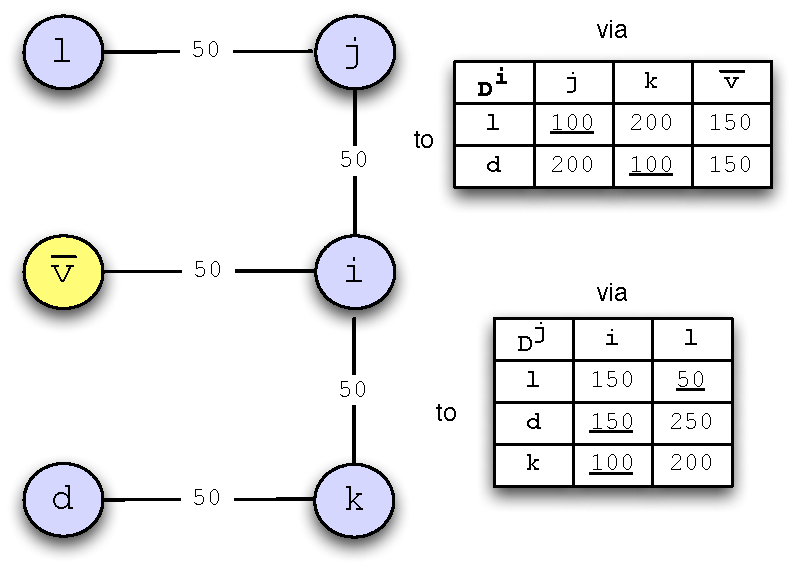
\includegraphics[scale=0.55]{figs/example-a-color.pdf}}
    \subfigure[After $\overline{v}$ is compromised. The dashed lines mark false paths claimed by $\overline{v}$.]
	{\label{fig:example-b}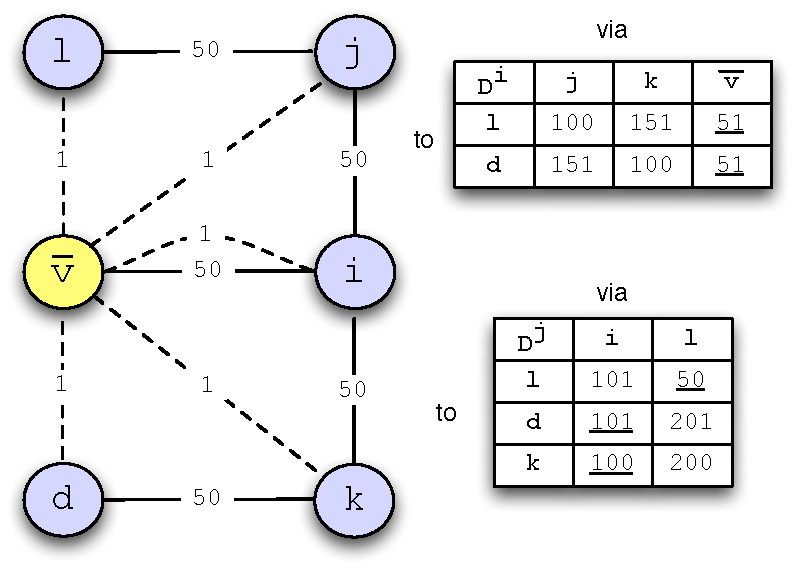
\includegraphics[scale=0.55]{figs/example-b-color.pdf}} 
    \subfigure[After recovery.]{\label{fig:example-c}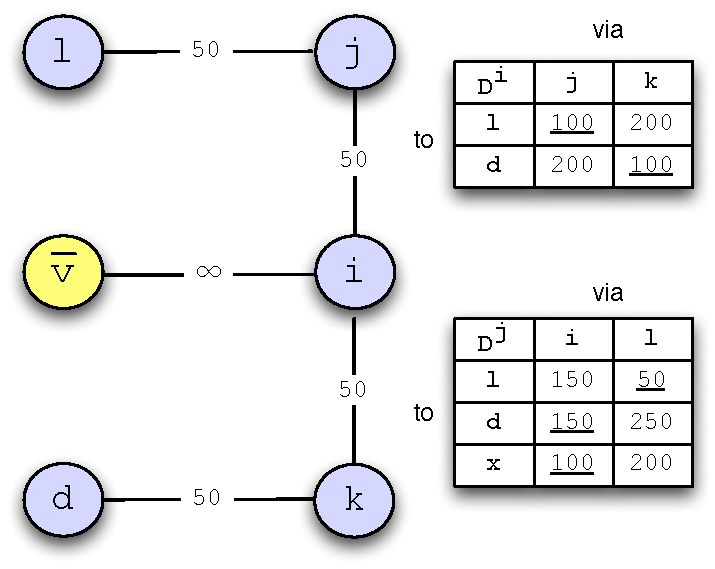
\includegraphics[scale=0.55]{figs/example-c-color.pdf}}
  \end{center}
	%\caption{Three snapshots of a graph, $G$.}
	\caption{Three snapshots of a graph, $G$, where $\overline{v}$ is the compromised node. Parts of $i$ and $j$'s distance matrix are displayed to the right of each sub-figure.
	The least cost values are underlined.}
	%$dmatrix_i$ and $dmatrix_j$ are displayed to the right of each sub-figure.
	%The least cost values are underlined.}
	%(a) $G$  before $\overline{v}$ is compromised, (b) $G$ after $\overrightarrow{bad}$ has}
	%has finished propagating but before recovery has started, and (c) $G$ after recovery. The dashed lines in (b) mark false paths used by $\overrightarrow{bad}$. 
	%Parts of $dmatrix_i$ and $dmatrix_j$ are displayed to the right of each sub-figure. The least cost values are underlined.}
  \label{fig:dv-example}
\end{figure*}


We trace the execution of \second using the example in Figure \ref{fig:dv-example}.
In Figure \ref{fig:example-b}, $i$ uses \bad to reach nodes $l$ and $d$.  $j$ uses $i$ to reach all nodes except $l$.  Notice that when $j$ uses $i$ to reach $d$, 
it transitively uses \badvector (e.g., uses path $j-i-$\bads$-d$ to $d$). 
After the preprocessing completes, $i$ selects a new neighbor to route through to reach $l$ and $d$ by finding its new smallest distance in \dmatrixi 
to these destinations: $i$ selects the routes via $j$ to $l$ with a cost of $100$ and $i$ picks the route via $k$ to reach $d$ with cost of $100$. 
(No changes are required to route to $j$ and $k$ because $i$ uses its direct link to these two nodes). 
Then, using traditional distance vector $i$ sends \minvi to $j$ and $k$.  When $j$ receives \minvis, $j$ must modify its distance to $d$ because \minvi indicates 
that $i$'s least cost to $d$ is now $100$.
$j$'s new distance value to $d$ becomes $150$, using the path $j-i-k-l$. $j$ then sends a message sharing \minvj with its neighbors.  From this point, recovery proceeds according 
by using traditional distance vector. 

%{\bf Pros/Cons.} 
\second is simple and makes no synchronization assumptions. % The primary advantage of \second is its simplicity.
However, \second is vulnerable to the \infinity problem. Because each node only has local information, the new shortest paths may continue to use \bads.
%When computing new shortest paths, a node cannot guarantee that the new shortest path does not use \bad because the node only has local information. 
For example, if $w(k,d)=400$ in Figure \ref{fig:dv-example}, a \infinity scenario would arise. After notification of \bads's compromise, 
$i$ would select the route via $j$ to reach $d$ with cost $151$ (by consulting \dmatrixis), using a path that does not actually exist in $G$ ($i-j-i-$\bads$-d$), since $j$ has removed \bad as a 
neighbor. When $i$ sends \minvi to $j$, $j$ selects the route via $i$
to $d$ with cost $201$. Again, the path $j-i-j-i-$\bads$-d$ does not exist.  In the next iteration, $i$ 
picks the route via $j$ having a cost of $251$. This process continues until each node finds their 
correct least cost to $d$.  We will see in our simulation study that the \infinity problem can incur significant message and time costs.




\subsection{The Purge Algorithm}
\label{subsec:purge}


\purge globally invalidates all false state using a diffusing computation and then uses distance vector to compute new distance values that avoid all invalidated paths.
Recall that diffusing computations preserve the decentralized nature of distance vector.
The diffusing computation is initiated at the neighbors of \bad because only these nodes are 
aware if \bad is used an intermediary node. The diffusing computations spread from \bads's neighbors to the network edge, invalidating false state at each node along the way. 
Then ACKs travel back from the network edge to the neighbors of \bads, indicating that the diffusing computation is complete. 
See Algorithm \ref{alg:purge} and \ref{alg:purge2} in the Appendix for a complete specification of this diffusing computation.

Next, \purge uses distance vector to recompute least cost paths invalidated by the diffusing computations.  In order to initiate the distance vector computation, each 
node is required to send a message after diffusing computations complete, even if no new least cost is found.  Without this step, distance vector may not correctly compute new least cost 
paths invalidated by the diffusing computations.  For example, consider the following the scenario when the diffusing computations complete: a node $i$ and all of $i$'s neighbors have 
least cost of $\infty$ to destination node $a$. Without forcing $i$ and its neighbors to send a message after the diffusing computations complete, neither $i$ nor $i$'s neighbors may
never update their least cost to $a$ because they may never receive a non-$\infty$ cost to $a$.

%{\footnote {\small The operations performed by the diffusing compuations described in Section \ref{subsec:preprocess} are  }
%This algorithm is specified in Algorithm \ref{alg:discover} of the Appendix.

In Figure \ref{fig:dv-example}, the diffusing computation executes as follows. First, $i$ sets its distance to $l$ and $d$ to $\infty$ (thereby invalidating $i$'s path to $l$ and $d$)
because $i$ uses \bad to route these nodes. Then, $i$ sends a message to $j$ and $k$ containing $l$ and $d$ as invalidated destinations.
When $j$ receives $i$'s message, $j$ checks if it routes via $i$ to reach $l$ or $d$. Because $j$ uses $i$ to reach $d$, $j$ sets its distance estimate to $d$ to $\infty$. 
$j$ does not modify its least cost to $l$ because $j$ does not route via $i$ to reach $l$. Next, $j$ sends a message that includes $d$ as an invalidated destination.
$l$ performs the same steps as $j$. After this point, the diffusing computation ACKs travel back towards $i$. When $i$ receives an ACK, the diffusing computation is complete. At this
point, $i$ needs to compute new least costs to node $l$ and $d$ because $i$'s distance estimates to these destinations are $\infty$. 
$i$ uses \dmatrixi to select its new route to $l$ (which is via $j$) and uses \dmatrixi to find $i$'s new route to $d$ (which is via $k$). Both new paths have cost $100$. Finally,
$i$ sends \minvi to its neighbors, triggering the execution of distance vector to recompute the remaining distance vectors.

Note that a consequence of the diffusing computation is that not only is all \badvector state deleted, but all \oldvector state as well.  
Consider the case when \bad is detected before node $i$ receives \badvectors.
It is possible that $i$ uses \oldvector to reach a destination, $d$. In this case, the diffusing computation will set $i$'s distance to $d$ to $\infty$.

An advantage of \purge is that it operates without the need for any clock synchronization.  We will find that \cprs, unlike \purges, either requires extra computation to maintain logical clocks or
assumes clocks are loosely synchronized. %no effort is required to synchronize clocks makes no synchronization assumptions. 
Also, \purges's diffusing computations ensure that the \infinity problem does not occur by removing
false state from the entire network. However, globally invalidating false state can be wasteful if valid alternate paths are locally available. 


\subsection{The CPR Algorithm}
\label{subsec:cpr}

\cprs {\footnote {\small The name is an abbreviation for {\bf C}heck{\bf P}oint and {\bf R}ollback. }} 
is our third and final recovery algorithm. 
Unlike \second and \purges, \cpr only requires that clocks across different
nodes be loosely synchronized i.e. the maximum clock offset between
any two nodes is assumed to be  bounded. For ease of explanation, we
describe \cpr as if the clocks at different nodes are perfectly
synchronized. Extensions to handle loosely synchronized clocks should
be clear. Accordingly, we assume that all neighbors of \bads, are
notified of the time, $t'$, at which \bad was compromised.  At the end of this section we comment on how the clock synchronization requirement assumption can be dropped by
using logical clocks.

For each node, $i \in G$, \cpr adds a time dimension to \minvi and \dmatrixis, which \cpr then uses to locally archive a complete history of values. 
Once the compromised node is discovered, 
the archive allows the system to rollback to 
a system snapshot from a time before \bad was compromised. From this point, \cpr needs to remove \bad and \oldvector and update stale distance values resulting from link weight changes.
We describe each algorithm step in detail. % (1) Create a \minv and \dmatrix archive. (2) roll back to a valid snapshot, and (3) steps after the rollback. 

{\bf Step 1: Create a \minv and \dmatrix archive.} 
	We define a  \emph{snapshot} of a data structure to be a copy of all current distance values along with a timestamp.
	{\footnote {\small In practice, we only archive distance values that have changed. Thus each distance value is associated with its own timestamp.}}
	The timestamp marks the time at which that set of distance values start being used. 
	\minv and \dmatrix are the only data structures that need to be archived. This approach is similar to ones used in temporal databases 
  \cite{Jensen91,Lomet06}.

  Our distributed archive algorithm is quite simple.  %For a given data structure, a node archives all current distance values whenever one of the values change. 
	Each node has a choice of archiving at a given frequency (e.g., every $m$ timesteps) or after some number of distance value changes (e.g., each time a distance 
	value changes).  Each node must choose the same option, which is specified as an input parameter to \cprs. A node archives independently of all other nodes.
  A side effect of independent archiving, is that even with perfectly synchronized clocks, the union of all snapshots may not constitute a globally consistent snapshot. 
  For example, a link weight change event may only have propagated 
  through part of the network, in which case the snapshot for some nodes will reflect this link weight change (i.e., among nodes that have learned of the event) 
  while for other nodes no local snapshot will reflect the occurrence of this event. We will see that a globally consistent snapshot is not required for correctness.  

{\bf Step 2: Rolling back to a valid snapshot.} 
Rollback is implemented using diffusing computations. Neighbors of the compromised node independently select a snapshot to roll back to, such that the snapshot is the most recent one taken
before $t'$.  Each such node, $i$, rolls back to this snapshot by restoring the \minvi and \dmatrixi values from the snapshot.  Then, $i$ initiates a diffusing computation to inform all other
nodes to do the same. If a node has already rolled back and receives an additional rollback message, it is ignored. 
(Note that this rollback algorithm ensures that no reinstated distance value uses \badvector because every node rolls back to a snapshot 
with a timestamp less that $t'$).  A pseudo-code specification of this rollback algorithm can be found in the Appendix (Algorithm \ref{alg:rollback}).  
%in the Appendix gives the pseudo-code for the rollback algorithm.


{\bf Step 3: Steps after rollback.} After Step 2 completes, the algorithm in Section \ref{subsec:preprocess} is executed.
There are two issues to address.
First, some nodes may be using \oldvectors.  Second, some nodes may have stale state as a result of link weight changes that occurred during $[t',t_b]$ and 
consequently are not reflected in the snapshot. 
To resolve these issues, each neighbor, $i$, of \bads, sets its distance to \bad to $\infty$ and then selects new least cost values that avoid the compromised node, triggering
the execution of distance vector to update the remaining distance vectors.  That is, for any destination, $d$, where $i$ routes via \bad to reach $d$,
$i$ uses \dmatrixi to find a new least cost to $d$. If a new least costs value is used, $i$ sends a distance vector message to its neighbors. Otherwise, $i$ sends no message.
Messages sent trigger the execution of distance vector.

During the execution of distance vector, each node uses the most recent link weights of its adjacent links. Thus, 
if the same link changes cost multiple times during  $[t',t_b]$, we ignore all changes but the most recent one. Algorithm \ref{alg:cpr} specifies Step 3 of \cprs.

In the example from Figure \ref{fig:dv-example}, the global state after rolling back is nearly the same as the snapshot depicted in Figure \ref{fig:example-c}:
the only difference between the actual system state and that depicted in Figure \ref{fig:example-c} is that in the former 
$(i,$\bads$)=50$ rather than $\infty$. Step 3 in \cpr makes this change.  Because no nodes use \oldvectors, no other changes take place.

Rather than using an iterative process to remove false state (like in \second and \purges), \cpr does so in one diffusing computation.
However, \cpr incurs storage overhead resulting from periodic snapshots of \minv and \dmatrixs.  Also, after rolling back, stale state may exist if link weight changes occur during $[t',t_b]$.
This can be expensive to update.
Finally, unlike \purge and \seconds, \cpr requires loosely synchronized clocks because without a bound on the clock offset, nodes may rollback to highly inconsistent local snapshots.
Although correct, this would severely degrade \cpr performance.

{\bf Using Logical Clock Timestamps.}
We can use Lamport's clock algorithm  \cite{Lamport78} to assign timestamps based on logical, rather than physical, clocks.  This allows us to drop the inconvenient assumption of loosely 
synchronized clocks. Here we briefly outline how the stated \cpr algorithm can be modified to use Lamport timestamps to create and restore system snapshots.

%First, \cpr is modified to create network-wide snapshots are periodically computed using diffusing computations instead of each node creating snapshots independently.   
First, \cpr is modified to create network-wide snapshots using diffusing computations instead of each node creating snapshots independently.   
Here each node records the logical timestamp when creating a checkpoint. 
The logical clock values are determined using the ``happened before'' relation defined by Lamport \cite{Lamport78}, where we limit events to be messages sent and received, and 
by piggybacking each node's logical clock value with each message it sends.  

%After being notified of \bads, each neighbor, $i$, of the compromised node determines the logical timestamp of the snapshot it wishes to restore.  
%This requires that either the detection algorithm specifies either \badvector or the logical time \bad was compromised. 
The second change to \cpr is in how each node determines the snapshot to restore during the roll back process (i.e., Step 2 above). Starting with each $i \in adj(\overline{v})$, 
$i$ determines the logical timestamp of the snapshot it wishes to restore.  This requires that the detection algorithm specifies either \badvector or the logical time \bad was compromised. 
In the latter case, finding the appropriate snapshot to restore is straightforward.
If only \badvector is provided, $i$ must additionally record each \minv vector received (as a part of standard distance vector messaging) 
along with the corresponding Lamport timestamp.  By doing so, this archive can be searched
to find the logical timestamp in which \badvector was first received at $i$.  Let $t_l$ denote this timestamp.  Next, $i$ initiates a diffusing computation instructing all other nodes 
to roll back to their most recent snapshot taken before $t_l$.  After this point, the diffusing computations continue as described in Step 2 above and Step 3 
remains unchanged.

Rolling back using logical timestamps does not guarantee that all \badvector state is removed because Lamport timestamps only provide partial ordering of events. 
With logical clocks, \cpr can be thought of as a best-effort approach to quickly removing false routing state by rolling back in time.  \cpr is still correct with logical clocks
for the reasons described in its correctness proof (Corollary \ref{cor:cpr-correct-single}).  
%This version of \cpr can be thought of as a best-effort approach to quickly removing false routing state.




\subsection{Multiple Compromised Nodes}
\label{subsec:mult}

Here we detail the necessary changes to each of our recovery algorithms when multiple nodes are compromised. Since we make the same changes to all three algorithms, we do not refer 
to a specific algorithm in this section. Let $\overline{V}$ refer to the set of nodes compromised at time $t'$. 

In the case where multiple nodes are simultaneously compromised, each recovery algorithm is modified such that for each $\overline{v} \in \overline{V}$, all $adj(\overline{v})$
are notified that \bad was compromised. 
%to accept a \emph{set} of compromised nodes, $\overline{V}$, as input (rather than a single node).  {\bf not really correct to refer to the set as input}
From this point, the changes to each algorithm are straightforward.  For example,
the diffusing computations described in Section  \ref{subsec:preprocess} are initiated at the neighbor nodes of each node in $\overline{V}$.
{\footnote {\small For \cprs, $t'$ is set to the time the first node is compromised.}}
%First, we augment the preceprocessing procedure described in Section \ref{subsec:preprocess}. In 
%the case where multiple nodes are simulataneously compromised, we modify the diffusing computations to remove all compromised nodes as a destination. %each of these nodes as a destination.

More changes are required to handle the case where an additional node is compromised during the execution of a recovery algorithm. Specifically, when another node is 
compromised, $\overline{v}_2$, we make the following change to the distance vector computation of each recovery algorithm.
{\footnote {\small {Recall that each of our recovery algorithms use distance vector to complete their computation.}} 
If a node, $i$, receives a distance vector message which includes a distance value to destination $\overline{v}_2$, then $i$ ignores said distance value and processes
the remaining distance values (if any exist) to all other destinations (e.g., where $d \neq \overline{v}_2$) normally.  If the message contains no distance information for any 
other destination $d \neq \overline{v}_2$, then $i$ ignores the message.
Because $\overline{v}_2$'s compromise 
triggers a diffusing computation to remove $\overline{v}_2$ as a destination, each node eventually learns the identity of $\overline{v}_2$, thereby allowing the node 
execute the specified changes to distance vector.

Without this change it is possible that the recovery algorithm will not terminate.  Consider the case of two compromised nodes, $\overline{v}_1$ and $\overline{v}_2$,
where $\overline{v}_2$ is compromised during the recovery triggered by $\overline{v}_1$'s compromise.  In this case, two executions of the recovery algorithm are triggered: one when
$\overline{v}_1$ is compromised and the other when $\overline{v}_2$ is compromised.
 Recall that all three recovery algorithms set all link weights to $\overline{v}_1$ to $\infty$ (e.g., $(v_i,\overline{v}_1)=\infty, \forall v_i \in adj(\overline{v}_1)$).
If the first distance vector execution triggered by $\overline{v}_1$'s compromise is not modified to terminate least cost computations to $\overline{v}_2$, the distance vector step of the 
recovery algorithm would never complete because the least cost to $\overline{v}_2$ is $\infty$. 






%%%%%%%%%%%%%%%% TRENDS IN RECOVERY SECTION %%%%%%%%%%
\section{Correctness of Recovery Algorithms}
\label{sec:correct}

Our correctness proofs consider the general case where multiple nodes are compromised. 
%We first state our assumptions and then define correctness. Finally, we prove the correctness of each algorithm. 
We assume the computation model described in Section \ref{sec:problem}.

\begin{define} 
An algorithm is correct if the following two conditions are satisfied. One, $\forall v \in V'$, $v$ has the least cost to all destinations $v' \in V'$.
Two, the least cost is computed in finite time.
\end{define}


\begin{theorem}
\label{thm:dv-correct}
Distance vector is correct.
\end{theorem}
\begin{proof}
Bertsekas and Gallager \cite{Gall87} prove correctness for distributed Bellman-Ford for arbitrary non-negative \dmatrix values. 
Their distributed Bellman-Ford algorithm is the same as the distance vector algorithm used in this paper. 
\end{proof}
%$Proof$. Bertsekas and Gallager \cite{Gall87} prove correctness for distributed Bellman-Ford for arbitrary nonnegative \dmatrix values. 
%Their distributed Bellman-Ford algorithm is the same as the distance vector algorithm used in this paper. \qed

\begin{corollary}
\label{cor:second-correct-single}
\second is correct when a single node is compromised.
\end{corollary}
\begin{proof}
As per the preprocessing step, each $v \in adj(\overline{v})$ initiates a diffusing computation to remove \bad as a destination. For each diffusing computation,
all nodes are guaranteed to receive a diffusing computation (by our reliable communication and finite graph assumptions). Further, each diffusing computation
terminates in finite time.  Thus, we conclude that each $v \in V'$ removes $\overline{v}$ as a destination in finite time.

After the diffusing computations to remove \bad as a destination complete, each 
$v \in adj($\bads$)$ uses distance vector to determine new least cost paths to all nodes in their connected component.
Because all \dmatrixv are non-negative for all $v \in V'$, by Theorem \ref{thm:dv-correct} we conclude \second is correct if no additional node(s) are compromised
during $[t',t^*]$. % the execution of \seconds. %trigger by the compromised of $\overline{V}$
\end{proof}

\begin{corollary}
\label{cor:second-correct-mult}
\second is correct when multiple nodes are compromised.
\end{corollary}
\begin{proof}
If multiple nodes, $\overline{V}$, are simultaneously compromised the proof is the same as that for Corollary \ref{cor:second-correct-single}, substituting $\overline{V}$ for $\overline{v}$.

Next, we prove \second is correct in the case where a set of nodes, $\overline{V}_2$, are compromised concurrent with a running execution of \second (e.g., during  $[t',t^*]$), triggered by the compromise of $\overline{V}$.
First we show that any least cost computation (e.g., one triggered by  $\overline{V}$'s compromise) to any $v \in \overline{V}_2$ is eventually terminated.  We have already proved that the diffusing computations to remove each $v \in \overline{V}_2$ as 
a destination complete in finite time.  Let $t_d$ mark the time these diffusing computations complete. For all $t \geq t_d$, any running least cost computation to a destination $v \in \overline{V}_2$ 
is terminated by the actions specified Section III-D of our Technical Report \cite{Tech}. %in Section \ref{subsubsec:mult}.  
Therefore, the only remaining least cost computations are to all $v \in V'$, where 
$V' = V - \left(\overline{V} \cup \overline{V}_2 \right)$.  Because all \dmatrixi values are non-negative for all $i \in V'$, by Theorem \ref{thm:dv-correct} we conclude \second is correct.
%when additional nodes are compromised concurrent with any \second execution. 
%We have already proved (in Corollary \ref{cor:second-correct-single}) that the diffusing computations to remove $\overline{V}_2$ as a destination complete in finite time.  

Since we have proved \second is correct when multiple nodes are simultaneously compromised and when nodes are compromised concurrent with any \second execution,
we conclude that \second is correct when multiple nodes are compromised.
\end{proof}


\begin{corollary}
\label{cor:purge-correct-single}
\purge is correct when a single node is compromised.
\end{corollary}
\begin{proof}
Each $v \in adj($\bads$)$ finds every destination, $a$, to which $v$'s least cost path 
uses \bad as the first-hop node. $v$ sets its least cost to each such $a$ to $\infty$, thereby invalidating its path to $a$.  
$v$ then initiates a diffusing computation. When an arbitrary node, $i$, receives a diffusing computation message from $j$, $i$ iterates 
through each $a$ specified in the message. If
$i$ routes via $j$ to reach $a$, $i$ sets its least cost to $a$ to $\infty$, therefore invalidating any path to $a$ with $j$ and  
\bad an intermediate nodes.  

%By our assumptions, each node receives a diffusing computation message and the diffusing computation terminates in finite time. Thus, we conclude that all paths using \bad as an intermediary
By our assumptions, each node receives a diffusing computation message for each path using $\overline{v}$ as an intermediate node.  Additionally, our assumptions imply that all
diffusing computation terminate in finite time. 
Thus, we conclude that all paths using $\overline{v}$ as an intermediary node are invalidated in finite time. 

Following the preprocessing, all $v \in adj($\bads$)$ use
distance vector to determine new least cost paths. Because all \dmatrixi are non-negative for all $i \in V'$, by Theorem \ref{thm:dv-correct} we conclude that \purge is correct. 
\end{proof}

\begin{corollary}
\label{cor:purge-correct-mult}
\purge is correct when multiple nodes are compromised.
\end{corollary}
\begin{proof}
The same proof used for Corollary \ref{cor:second-correct-mult} applies for \purges.
\end{proof}

\begin{corollary}
\label{cor:cpr-correct-single}
\cpr is correct when a single node is compromised.
\end{corollary}
\begin{proof}
\cpr sets $t'$ to the time $\overline{v}$ was compromised. Then, \cpr rolls back using diffusing computations: each diffusing computation is initiated at each $v \in adj(\overline{v})$.
Each node that receives a diffusing computation message, rolls back to a snapshot with timestep less than $t'$.
By our assumptions, all nodes receive a message and the diffusing computation terminates in finite time.  Thus, we conclude
that each node $v \in V'$ rolls back to a snapshot with timestamp less than $t'$ in finite time.

\cpr then runs the preprocessing algorithm described in Section \ref{subsubsec:preprocess}, which removes each \bad as a destination in finite time (as shown
in Corollary \ref{cor:second-correct-single}). Because each node rolls back to a snapshot in which all least costs are non-negative and 
\cpr then uses distance vector to compute new least costs, by Theorem $1$ we conclude that \cpr is correct if no additional nodes are compromised during  $[t',t^*]$.
\end{proof}

\begin{corollary}
\label{cor:cpr-correct-mult}
\cpr is correct when multiple nodes are compromised.
\end{corollary}
\begin{proof}
If multiple nodes, $\overline{V}$ are simultaneously compromised, \cpr sets $t'$ to the time the first $\overline{v} \in \overline{V}$ is compromised.  Any nodes, $\overline{V}_2$, compromised
concurrent with $\overline{V}$ (e.g., during  $[t',t^*]$), trigger an additional \cpr execution.  The steps described in Section \ref{subsec:mult} ensure 
that all least cost computations (after rolling back) are to
destination nodes $a \in V'$.  By Theorem \ref{thm:dv-correct} we conclude \cpr is correct because all \dmatrixi are non-negative for all $i \in V'$.
\end{proof}










\section{Analysis of Algorithms}
\label{sec:analysis}

In this section we find communication complexity bounds for each recovery
algorithm (Section \ref{subsec:complex}). All proofs assume a synchronous model in which nodes send and receive messages at fixed epochs. 
In each epoch, a node receives a message from all its neighbors and performs its local computation. In the next epoch, the node sends a message (if needed). 
%All algorithms are deterministic under this communication model. The synchronous communication model, although simple, yields interesting insights into the performance of each of the recovery algorithms.


\subsection{Communication Complexity}
\label{subsec:complex}

We derive communication complexity bounds for each recovery algorithm. First, we consider graphs where link costs remain fixed
(Section \ref{subsub:diffuse-complex} - \ref{subsubsec:purge-analysis}). Then, we derive bounds where link costs can change (Section \ref{subsubsec:linkchange-complex}).

We make the following assumptions in our complexity analysis:
\begin{itemize}
	\item There is only a single compromised node, \bads.
	\item We assume all nodes have unit link cost of $1$ and that \bad falsely claims a cost of $1$ to each $j \in V'$ (e.g., $\forall j \in V', \delta_s(\overline{v},j) = 1$).
	\item Since we assume unit link costs of $1$, a link cost increase correspond to the removal of a link and a link cost decrease corresponds to the addition of a link.
\end{itemize}

\subsubsection{Diffusing Computation Analysis}
\label{subsub:diffuse-complex}

We begin our complexity analysis with a study of the diffusing computations common to all three of our recovery algorithms: \seconds, \cprs, and \purges. 
In our analysis, we refer to $a$ as our generic destination node.  

\begin{lemma}
\label{lem:diffuse}
%Each diffusing computation has $O(n^2)$ message complexity.
Each diffusing computation has $O(E)$ message complexity.
\end{lemma}

\begin{proof}
Each node in a diffusing computation sends a query to all downstream nodes and a reply to its parent node. 
Thus, no more than $2$ messages are sent across a single edge, yielding $O(E)$ message complexity.
%Since a node can have at most $n-2$ downstream nodes and only $1$ parent node, the communication overhead for each diffusing computation message is $O(n^2)$.
\end{proof}


\begin{theorem}
\label{lem:diffuse-total}
%The diffusing computations for \seconds, \cprs, and \purge have $O(n^3)$ communication complexity.
The diffusing computations for \seconds, \cprs, and \purge have $O(mE)$ communication complexity.
\end{theorem}

\begin{proof}
For each algorithm, diffusing computations are initiated at each $i \in adj(\overline{v})$, so there can be at most $m$ diffusing computations. 
From Lemma \ref{lem:diffuse}, each diffusing computation has $O(E)$ 
communication complexity, yielding $O(mE)$ communication complexity. %for diffusing computations used by \seconds, \cprs, and \purges. 
\end{proof}


\subsubsection{\second Analysis}
\label{subsubsec:second-analysis}


%{\bf summary of graph and similarity of DV and \seconds} \\
Johnson \cite{Johnson84} studies DV over topologies with bidirectional links and unit link costs of $1$.  Specifically, Johnson analyzes DV update 
activity after the failure of a single network resource, in which a resource is either a node or a link.  She assumes that nodes adjacent to a failed resource detect 
the failure and then react according to DV: in the case of a failed node, each node sets its distance to the failed node to $n$ and no link connected to the 
failed node is used in the final correct shortest paths. 
{\footnote {\small {The maximum distance to any node under Johnson's model is $n$, where $n$ is the number of nodes in the graph. This is equivalent to $\infty$ in our case.}}
From this point, DV behaves exactly like \seconds.
%After the failure of a resource is detected, DV behaves exactly like \seconds.
{\footnote {\small Note that in contrast to Johnson, we assume an outside algorithm identifies the compromised node.}}
Therefore, by mapping our false path problem to Johnson's failed resource problem, we can use Johnson's analysis of DV to find bounds (and exact message counts) for \seconds.
%Therefore, by mapping Johnson's failed resource problem to our false path scenario, we can use Johnson's analysis of DV to find bounds (and exact message counts) for \seconds.
To do so, we modify the graph, $G$, that Johnson considers by adding false paths between \bad and all other nodes.
%In the single destination case, we introduce a false path from \bad to $a$, where $a$ is the generic destination.  
%Likewise, for the multiple destination scenario, false paths are introduced between \bad and all other nodes.

%Thus, Johnson's analysis applies directly to \second if we introduce a false path from \bad to $d$, in the single destination case, and false paths between \bad and 
%all other nodes, in the multiple destination scenario.
%In summary, because DV behaves the same as \second after the failed node or compromised node is identified, respectively, we can apply Johnson's analysis of DV to find bounds 
%(and even exact message counts) on \second performance. 
%For example,when a node $x$ detects the failure of an adjacent node $y$, $x$ sets its distance to $y$ to $n$
%which triggers the execution of DV.  

%This is precisely the behavior of \seconds, except that in our case we assume an outside algorithm identifies the compromised node, while Johhnson
%assumes that each node can detect the failure of adjacent link and/or node. 

In Corollary \ref{cor:during}, we proved that with \second nodes using \bad as an intermediate node count up from an initial incorrect least costs to their final correct value.  
Johnson proves the same for DV. 
Using this pattern, Theorem \ref{thm:second-lbub} derives upper and lower bounds for \seconds.  Intuitively, the lower bound occurs when nodes count up by $2$ (to their final correct
value) and the upper bound results when nodes count up by $1$. 


\begin{theorem}
\label{thm:second-lbub}
After $\hat{t}$, \second message complexity is bounded below by 
\begin{eqnarray}
\label{thm:second-lb}
\sum_{i \in V'} \Big\lceil  \frac{\max_{j \in V', i \neq j} \left( C(i,j) \right)}{2}  \Big\rceil adj(i)
%\sum_{i \in V'} \max \left( \sum_{j \in V', i \neq j} \Big\lceil \frac{C(i,j)}{2}\Big\rceil \right) adj(i)
\end{eqnarray}
and above by 
\begin{eqnarray}
\label{thm:second-ub}
\sum_{i \in V'} \max_{j \in V', i \neq j} \left( C(i,j) \right) adj(i)
%\sum_{i \in V'} \max \left( \sum_{j \in V', i \neq j} C(i,j) \right) adj(i)
\end{eqnarray}
\end{theorem}

\begin{proof}
Theorem 2 from \cite{Johnson84} gives a lower bound of $\displaystyle \sum_{i,j \in V', i \neq j} \Big\lceil  \frac{1}{2} C(i,j)  \Big\rceil adj(i)$. 
However, this lower bound applies to a version of 
DV in which each message contains update costs for only a single destination; in a single epoch, if a node finds new least costs to multiple destinations, 
a separate message is sent for each destination with a new least cost (and is sent to each of the node's neighbors).
In contrast, \second handles updates to multiple destinations concurrently: in each epoch, a single message sent by node $i$ contains new distance values for all destinations in which $i$ has 
a new least cost. For this reason, the maximum $C(i,j)$ value determines the number of times a node sends a message to each neighbor node. 

%Since least cost computations for all destinations are handled conccurently, for \seconds the maximum $C(i,j)$ value 
%yields a lower bound on the number of times a node sends a message to each neighbor node. 
%In contrast to the version of DV considered by Johnson \cite{Johnson83} -- which, at each epoch, nodes send a seperate message for updates to each destination -- at each epoch, \second handles updates to multiple destinations concurrently (e.g., sends updates for multiple destinations with a single message).  For this reason, the maximum $C(i,j)$ value determines the number of times a node sends a message to each neighbor node. 

The upper bound (Equation \ref{thm:second-ub}) is also derived from Theorem 2 in \cite{Johnson84}.  Theorem 2 gives us a upper bound of 
$\displaystyle \sum_{i,j \in V', i \neq j} C(i,j) \cdot adj(i)$. For the same reason described for the lower bound, the maximum $C(i,j)$ value determines the number of times a node sends a message to each neighbor node.
%we take the maximum $C(i,j)$ to derive an upper bound on message complexity.
\end{proof}

\begin{corollary}
\label{cor:second-bigo}
%\second sends $O(n^2d)$ messages.
\second has $O(mnd)$ communication complexity.
\end{corollary}
\begin{proof}
From Lemma \ref{lem:diffuse-total}, \seconds's diffusing computations have $O(mE)$ communication complexity. Next, \second runs DV. 
It must be the case that $C(i,j) \leq d$ and each node can at most have $m$ neighbors.  Since $|V'| = n-1$, DV and therefore \second has $O(mnd)$ communication complexity.
%We conclude that \second has $O(mnd)$ communication complexity.
%$c \times n \times n \times d$, where $c = \{\frac{1}{2},1\}$.  Thus, \second sends $\Theta(n^2d)$ messages.
\end{proof}

Next, we restate Theorem 1 from Johnson \cite{Johnson84} using our notation.  Theorem \ref{thm:second-allpaths} introduces the term \emph{allowable path}.
An allowable path from node $i$ to \bad is a path in the original network ($G$) from node $i$ to \bad which does not use \bad as an intermediate node.

\begin{theorem}
\label{thm:second-allpaths}
Each incorrect route table entry assumes all possible lengths of paths of the form $|P| + \delta_s(\overline{v},a)$ where $P$ is an allowable path from node $i$ to \bad and 
$\delta_s(\overline{v},a)$ is the length of the false path claimed by \bads.
\end{theorem}

Theorem \ref{thm:second-allpaths} translates the problem of finding the number of update messages after false node detection into the problem of finding all possible 
allowable paths between each node $i$ and \bads.  By doing so, we can find the exact number of messages required for \second recovery.
%Johnson states that if there exists an allowable path between $i$ and \bad of length $p$, then there exists an allowable path
%of length $p + 2i$ from $i$ to \bads, for all non-negative values of $i$.  These paths are derivived by hopping back and forth between $i$ and an adjacent node $j$ (where $j \neq$ \bads) 
%$i$ times and then finally using the path of length $p$ from $i$ to \bads.

The next two theorems, Theorem \ref{thm:second-even} and \ref{thm:second-odd}, follow from Theorem 5 in \cite{Johnson84} and Theorem \ref{thm:second-allpaths}.

\begin{theorem}
\label{thm:second-even}
If $G$ contains no odd cycles, the number of update messages after $\hat{t}$ is described exactly by Equation \ref{thm:second-lb}.
%\begin{eqnarray}
%\sum_{i \in V'} \max \left( \sum_{j \in V', i \neq j} \Big\lceil \frac{C(i,j)}{2}\Big\rceil \right) adj(i)
%\end{eqnarray}
\end{theorem}

Define $S(p)$ to be the set of nodes such that if $i \in S(p)$ there exists an allowable path of length $p$ and $p+1$ from $i$ to \bads. 
Let $q(\overline{v},i)$ be the smallest positive integer $p$ such that $i \in S(p)$ and $q(\overline{v},i)=c$.
%Let $S = \bigcup_{p=1}^\infty S(p)$ and $q(\overline{v},i)$ be the smallest positive integer $p$ such that $i \in S(p)$, and $\infty$ otherwise.
%Finally, for an arbitrary node $i \neq \overline{v}$, let $q(\overline{v},i)=c$.
%Define a node $i$ to singular if $i \in S(p)$ for some $p$.  
%Let $S = \bigcup_{p=1}^\infty S(p)$. If $i \notin S$, then $i$ is nonsingular. Finally, let $q(\overline{v},i)$ be the smallest positive integer $p$ such that $i \in S(p)$, if 
%$i$ is singular, and $\infty$ otherwise. %Let $q(\overline{v},i) = s$. 

\begin{theorem}
\label{thm:second-odd}
%If $G$ contains an odd cycle, for arbitrary $i,a \in V'$  if $c + \delta_s(\overline{v},a) < \delta_f(i,a)$, then $\delta(i,a)$ increase in length by increments of $2$ until reaching the 
If $G$ contains an odd cycle and $c + \delta_s(\overline{v},a) < \delta_f(i,a)$, then allowable paths to \bad increase in length by increments of $2$ until reaching the 
value $c$ and then increments by $1$ thereafter.  Thus, the number of changes in $\delta(i,a)$, after $\hat{t}$, is:
\begin{eqnarray}
C(i,a) - \frac{1}{2} \displaystyle \left(c - \delta_s(i,a)\right)
\end{eqnarray}
If $c + \delta_s(\overline{v},a) \geq \delta_f(i,a)$, then update activity ceases before node $i$'s least cost entries begin to increase by $1$.  Thus, in this case the number of update messages, after $\hat{t}$, is
described exactly by Equation \ref{thm:second-lb}.
%$\displaystyle \sum_{i \in V'} \max \left( \sum_{j \in V', i \neq j} \Big\lceil \frac{C(i,j)}{2}\Big\rceil \right) adj(i)$.
\end{theorem}


Theorem \ref{thm:second-allpaths} tells us that before converging on the correct distance to a destination, $a$, \second exhaustively searches all paths from $i$ to \bad and then uses \bad's
false path to $a$.  If $G$ contains no odd cycle, then $i$ counts up by $2$ until reaching the final correct cost to $a$. Node $i$ does so by hopping back and forth between an adjacent node $j$ 
(where $j \neq$ \bads) $k$ times (for some integer $k \geq 0$), then uses an allowable path from $i$ to \bads, and finally uses \bad's false path to $a$.

However, if $G$ contains an odd cycle then the update behavior is slightly more complicated.  Node $i$ counts up by $2$ until $\delta(i,a)$ reaches a specific value, $c^*$, at which point, $i$ counts 
up by $1$ until $i$ converges on the final correct distance to $a$.  In Figure \ref{fig:second-odd}, $c^* = \delta(i,h) + \delta(h,\overline{v}) + \delta_s(\overline{v},a) = 1 + (p-1)+1 = p+1$.
In the epoch after $\delta(i,a)$ is set to $c^*$, node $i$ uses its path via $h$ of length $p$ to \bad (and then \bads's false path to $a$).
In the following epoch, $i$ uses its path via $l$ of length $p+1$ to \bads.  
From this point, $i$ counts up by $1$ by using allowable paths of lengths $p+2k$, for integer $k \geq 1$, (by hopping back and forth between $h$) to \bad and allowable paths of length $(p+1)+2k$ 
(by ping-ponging with $l$) to \bads, until $\delta(i,a)$ counts up to $\delta_f(i,j)$.
%For this reason, once $\delta_t(i,j) = c$, $i$ counts up by $1$.

%$c^* = c + \delta_s(\overline{v},a)$.  When $\delta(i,a) < c^*$, $i$ counts up by $2$ by hopping back and forth between an adjacent
%node.  When $\delta(i,a) \geq c^*$, $i$ can use a path of length $p$ to \bads.


\begin{figure}[t]
\centering
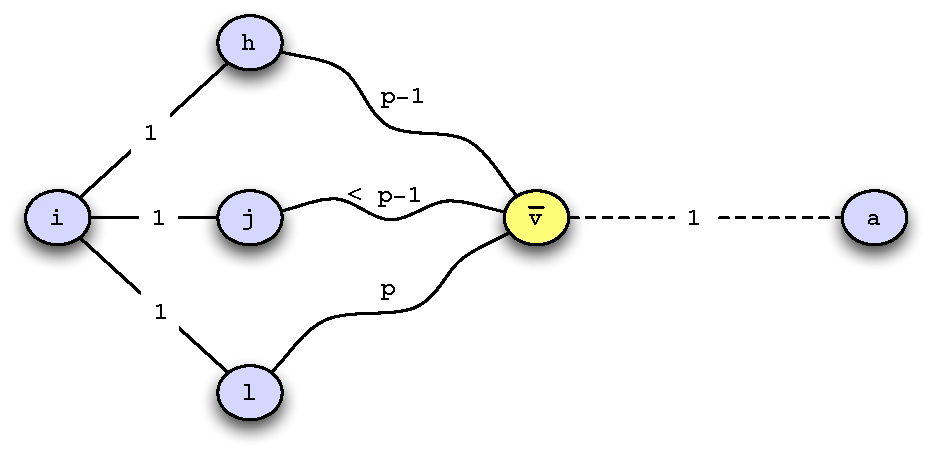
\includegraphics[scale=.57]{figs/second-odd.pdf}
\caption{The yellow node (\bads) is the compromised node.  The dotted line from \bad to $a$ represents the false path. }
\label{fig:second-odd}
\end{figure}

%Intuitively, Theorem \ref{thm:second-odd} establishes that for each destination, $a$, node $i$ counts up by $2$ until reaching value $c$. 
%Node $i$ does so by using allowable paths of length $p^* + 2k$ -- 
%for integers $k \geq 0$ and where $p^*$ is the minimum length path from $i$ to \bad -- and then by uses \bads's false path to destination $a$. 
%These $p^* + 2k$ length paths are derived by hopping back and forth between node $i$ and an adjacent node $j$ 
%(where $j \neq$ \bads) $k$ times and then finally using the path of length $p^*$ from $i$ to \bads.  
%After counting up to $c$ (e.g., when $i$'s least cost to $a$ is $c$), in the next epoch, $i$ uses its path of length
%$p$ to \bads. In the following epoch, $i$ uses its path of length $p+1$ to \bads.  
%From this point, $i$ uses allowable paths of lengths $p+2k$ and $(p+1)+2k$ to \bads, until counting up to $\delta_f(i,j)$.
%For this reason, once $\delta_t(i,j) = c$, $i$ counts up by $1$.



\subsubsection{\cpr Analysis}
\label{subsubsec:cpr-analysis}

The analysis for \second applies to \cpr because after rolling back \cprs, executes the steps of \seconds.  In fact, because \cpr performs the rollback 
using the same diffusing computations analyzed for \second (e.g., the diffusing
computations that remove \bad as a destination), the results for \second apply to \cpr with no changes. %analysis is required for \cprs.  

Although Theorem \ref{thm:second-lbub}, Theorem \ref{thm:second-even}, and Theorem \ref{thm:second-odd} apply directly to \cprs, the bounds and exact message count can defer 
between \second and \cprs. 
%We have already proved in our Technical Report \cite{Tech}, for \cprs, that all nodes correctly rollback to a checkpoint taken before \bad is compromised.  
%Let $\hat{t}$ mark the time \cprs's diffusing computations (to rollback) complete. 
%Because \cpr runs \second at $\hat{t}$, we redefine $C(i,j)$ for \cpr as $C(i,j) = \delta_f(i,j) - \delta_{\hat{t}}(i,j)$.	 
In most cases,  $\delta_{\hat{t}}(i,j)$ for \second is smaller than $\delta_{\hat{t}}(i,j)$ for \cpr because \cpr rolls back to a checkpoint taken before \bad is compromised. 
{\footnote {\small At worst, $\delta_{\hat{t}}(i,j)$ is equivalent across \second and \cprs.  This occurs when the false least vector claimed by \bad matches the least cost
vector used by \bad before being compromised (e.g., \badvectors$=$\oldvectors). }}
Thus, \cprs's $C(i,j)$ values are typically smaller than those for \seconds, resulting in lower message complexity for \cprs.

\subsubsection{\purge Analysis}
\label{subsubsec:purge-analysis}

Our \purge analysis establishes that after the diffusing computations complete, all nodes using false routing state to reach a destination
have a least cost of $\infty$ to this destination.  %Then, control moves back to the neighbors of the compromised node (becausee diffusing computations are initiated from these nodes)
From this point, these least costs remain $\infty$ until updates from nodes with a non-infinite cost to the destination spread through the network.  Upon receiving a non-infinite
least cost to the destination, nodes switch from an infinite least cost to a finite one (Lemma \ref{lem:purge-shrink}).  We establish that the first finite cost to the destination is in fact the node's final correct
least cost to the destination (Theorem \ref{thm:purge-oneupdate}). In this way, least costs change from $\infty$ to their final correct value.
%These correct least costs spread throughout the network until all nodes receive a correct least cost to the destination. % at which point \purge converges
%The correct least costs spread throughout the network and \purge converges on correct least costs when all nodes have received a finite least cost.

In the presence of a tie, we assume a node uses the least cost path that avoids \bads. Note that if ties are broken by using the path with \bad as intermediate node, our
proofs still apply, although with a few minor changes. 
Now we are ready to define two sets that are key structures in our \purge proofs.

\begin{define}
Let $B(a,t)$ be the set of nodes that have least cost $\infty$ to destination node $a$ at time $t$. %$\hat{t}$. %of nodes that have least cost $\infty$ at time $\hat{t}$.
\end{define}

\begin{define}
$F(a,t)$ is the set of nodes such that if $b \in F(a,t)$ then the following must be true:
%$F(a)$ is the set of nodes such that if $b \in F(a)$ then the following must be true at $\hat{t}$:
\begin{enumerate}
	\item $b \notin B(a,t)$.

	\item $\exists b': b' \in adj(b) \wedge b' \notin B(a,t)$.
	%\item $\exists v_{i'j'}: v_{i'j'} \in adj(v_{ij}) \wedge v_{i'j'} \notin B(0)$.
	
	\item $\exists b'': b'' \in adj(b) \wedge b'' \in B(a,t)$.
	%\item $\exists v_{i'j'}: v_{i'j'} \in adj(v_{ij}) \wedge v_{i'j'} \in B(0)$.

\end{enumerate}
\end{define}
%$\forall v_{ij} \in F, \exists v_{i'j'}: v_{i'j'} \in adj(v_{ij}) \wedge v_{i'j'} \notin B(0)$. %$ has $v_j \in adj(v_i): v_j \notin B(0)$. 
% $F$ is the set of all nodes, $v_{ij}$ such that $v_{ij} \notin B(0)$ and 

%\lemma{For an arbitrary $b \in F$ and $a \in V'$, $\ell(b,\overline{v}) = \{\ell(b,a) - 1, \ell(b,a) - 2 \}$

Next, in Lemma \ref{lem:purge-shrink} we prove that the size of $B(a,t)$ shrinks by at least one for each timestep beginning with $t''$ -- where
$t''$ refers to the time that the first $i \in V'$ with $\delta(i,a) = \infty$ changes $\delta(i,a)$ to a finite value -- until $B(a,t)$ is empty.
%This continues until $B(a,t)$ is empty.

\begin{lemma}
\label{lem:purge-shrink}
For each $t \geq t''$, $|B(a,t)| \geq |B(a,t+1)| + 1$, until $B(a,t) = \emptyset$.
%in each subsequent timestep until $B(a) = \emptyset$ at least one node, $j$, changes $\delta(j,a)$ from $\infty$ to a finite value after $\hat{t}$.
\end{lemma}
\begin{proof}
Once \purge diffusing computations complete at $\hat{t}$, a DV computation is triggered at each $v \in adj(\overline{v})$. 
At this point, all least costs corresponding to paths using \bad as an intermediate node are set to $\infty$ (this is proved in Corollary \ref{cor:purge-correct-single}).
As such, each $i \in B(a,\hat{t})$ sends a DV message
with a least of $\infty$ to each neighbor, {\footnote {\small Recall that after $\hat{t}$, \purge forces each node to send a least cost message to each neighbor 
(even if the node's least cost has not changed since $\hat{t}$). }} 
unless $i$ has a neighbor node in $F(a,\hat{t})$ (note that we denote this time as $t''$). 
In this case, $i$ selects a finite least to $a$ (which implies $i \notin B(a,t'')$), triggering the propagation of finite least costs to $a$.  Specifically, in each 
subsequent timestep $t$ (until $B(a,t) = \emptyset$) at least one node, $j$, changes $\delta_t(j,a)$ from $\infty$ to a finite value.  This is the case because unless $B(a,t) = \emptyset$, 
a node $i$ that has changed $\delta_t(i,a)$ from $\infty$ to a finite value, has $j \in adj(i)$ with $\delta_{t}(j,a) = \infty$ and thus $\delta_{t+1}(j,a)$ will be finite.  
A finite $\delta_{t+1}(j,a)$ value implies $j \notin B(a,t+1)$. Since $B(a,t)$ is monotonic, eventually $B(a,t) = \emptyset$. 
%subsequent timestep, $t: t < t^*$, at least one node, $j$, changes $\delta(j,a)$ from $\infty$ to a finite value.  This is the case because at $t-1$, a node $i$ that has changed 
\end{proof}

Our next Lemma (\ref{lem:purge-pathlen}) lists all possible values for the number of links between any $b \in F(a,\hat{t})$ and \bads.  We later use this Lemma in
Theorem \ref{thm:purge-oneupdate}.

\begin{lemma}
\label{lem:purge-pathlen}
For all $b \in F(a,\hat{t})$, $\ell(b,\overline{v}) = \{\ell(b,a), \ell(b,a) - 1\}$.
\end{lemma}
\begin{proof}
Let $b$ be an arbitrary node in $F(a,\hat{t})$.
If $\ell(b,\overline{v}) < \ell(b,a) -1$, this would imply $b \in B(a,\hat{t})$, a contradiction (a violation of condition $1$ of the $F(a,\hat{t})$ definition).  
On the other hand, consider the case where $\ell(b,\overline{v}) > \ell(b,a)$ and where $b' \in adj(b)$ and $b' \in B(a,\hat{t})$.  
Any path $b'$ uses with \bad as an intermediate node has cost
%If $\ell(b,\overline{v}) > \ell(b,a)$ then at $\hat{t}$, $b'$ can use $b$ as a next-hop router with $\delta_{\hat{t}}(b',a)=  \ell(b,a) +1$.  
%While any path $b'$ uses with \bad as an intermediate node has cost
$\ell(b,\overline{v}) -1 + \delta_s(\overline{v},a)  = \ell(b,\overline{v}) -1 + 1 =  \ell(b,\overline{v})$.  Since we have assumed $\ell(b,\overline{v})> \ell(b,a)$,
$b'$ would use $b$ as a next-hop router along $p_{\hat{t}}(b',a)$. 
%{\footnote {\small Note that if $b'$ routes via another node, $b''$, such that $b'' \neq b \wedge b'' \in F(a,\hat{t})$, this would imply $b'' \notin B(a,\hat{t}$. }}
This implies $b'\notin B(a,\hat{t})$, a contradiction. 
\end{proof}

The following theorem is the key argument in establishing \purges's communication complexity.  Theorem \ref{thm:purge-oneupdate} proves that once any $i \in V'$ changes its least cost 
from $\infty$, $i$ changes its least cost to the final correct value.

\begin{theorem}
\label{thm:purge-oneupdate}
For $t > \hat{t}$ and an arbitrary destination $a \in V'$, each $i \in B(a,\hat{t})$ with $\delta_{\hat{t}}(i,a) = \infty$ only modifies $\delta(i,a)$ once,
such that $\delta(i,a)$ changes from $\infty$ to $\delta_f(i,a)$.
\end{theorem}
\begin{proof}
Consider an arbitrary $i \in V'$ such that $i \in B(a,\hat{t})$. $i$ must use some $b \in F(a,\hat{t})$ as an intermediate node along $p_f(i,a)$. % where $a$ is an arbitrary destination.
Let $b^*$ be this node. % (e.g., $b^* \in F(a)$ such that $b^*$ used along $p_f(i,a)$). 
If we show that $\delta_f(b^*,a)$ is the first least cost among all $b \in F(a,\hat{t})$ to reach $i$,
then we have proved our claim because in Lemma \ref{lem:purge-shrink} we proved that $i$ does not update its least cost to a finite value until it receives a least cost from a $b \in F(a,\hat{t})$.
{\footnote {\small  Note that any node $i$ with $\delta(i,a) = \infty$ only changes $\delta(i,a)$ to a finite value. Thus, when \purge forces 
nodes to send a message after $\hat{t}$ to initiate the DV computation, no $i \in B(a,\hat{t})$ receiving a least cost of $\infty$ updates its least cost.}}
For the sake of contradiction, assume that for some $b' \in F(a,\hat{t})$, where $b' \neq b^*$, that $\delta_f(b',a)$ reaches $i$ before $\delta_f(b^*,a)$. 
{\footnote {\small From Lemma \ref{lem:purge-shrink} we know that a finite least cost to $a$ reaches every node in $B(a,\hat{t})$.}}
%{\footnote {\small It is easy to show by induction for an arbitrary $b \in F(a,\hat{t})$ that once a $b' \in adj(b)$,
%modifies for $\delta_t(b',a)$ from $\infty$ to a non-infinite value, that each subsequent timestep, $t < t^*$, at least one node changes its least cost from $\infty$ to a non-infinite value. }}
This implies that:
\begin{eqnarray}
\label{eqn:fcont}
\ell(b',\overline{v}) + \ell(i,b')  &<& \ell(b^*,\overline{v}) + \ell(i,b^*) 
\end{eqnarray}

From Lemma \ref{lem:purge-pathlen}, we know that $\ell(b',\overline{v}) = \{\ell(b',a), \ell(b',a) - 1\}$ and  $\ell(b^*,\overline{v}) = \{\ell(b^*,a), \ell(b^*,a) - 1\}$ 
%It must be the case that $\ell(b',\overline{v}) + 1 = \ell(b',d)$ and $\ell(b^*,\overline{v}) + 1= \ell(b^*,d)$. 
%The other possibility is that $\ell(b',\overline{v}) + 1 = \ell(b',d)$ and $\ell(b^*,\overline{v}) +1 = \ell(b^*,d)$.  
If we substitute  $\ell(b',\overline{v}) = \ell(b',a)$ and $\ell(b^*,\overline{v}) = \ell(b^*,a)$ into Equation \ref{eqn:fcont}, it yields:
\begin{eqnarray}
\label{eqn:purge-contr1}
\ell(b',a) + \ell(i,b')  &<& \ell(b^*,a) + \ell(i,b^*) 
%\ell(i,b') + \ell(b',a) &<& \ell(i,b^*) + \ell(b^*,a) 
\end{eqnarray}
However, since we have assumed that $i$ routes via $b^*$, we know that: 
%This is a contradiction because, we have assumed that $i$ routes via $b^*$, which implies:
\begin{eqnarray}
\label{eqn:purge-contr2}
  \ell(b',a) + \ell(i,b')  &>& \ell(b^*,a) +  \ell(i,b^*) 
  %\ell(i,b') + \ell(b',a) &>&  \ell(i,b^*) + \ell(b^*,a) 
 \end{eqnarray}
Thus, between Equation \ref{eqn:purge-contr1} and Equation \ref{eqn:purge-contr2} we have a contradiction.
Similar contradictions can be derived by substituting all other permutations of the $\ell(b',\overline{v})$ and $\ell(b^*,\overline{v})$ equalities, derived from Lemma \ref{lem:purge-pathlen}.
In conclusion, we have shown by contradiction that $\delta(i,a)$ only changes a single time: $\delta(i,a)$ changes from $\infty$ to $\delta_f(i,a)$.
\end{proof}


\begin{corollary}
\label{cor:purge-loopfree}
\purge is loop-free at every instant of time.
\end{corollary}

\begin{proof}
Before $\hat{t}$, only diffusing computation run. Diffusing computations are loop-free because computation proceeds along spanning trees, which are by definition acyclic. 
After $\hat{t}$, only DV computations run. From Theorem \ref{thm:purge-oneupdate} we know that each node with least cost $\infty$ to an arbitrary destination, changes its least cost once:
from $\infty$ to the correct final least cost. We conclude that \purge is loop free.
\end{proof}

%\begin{proof}
%After the diffusing computations complete, all $\delta(i,j)$ values are either correct or $\infty$.  Jaffe and Moss \cite{JaffMoss} prove 
%DV is loop-free for these exact start conditions.  Since \purge runs
%DV after the diffusing computations complete, we conclude that \purge is loop-free.
%\end{proof}

\begin{theorem}
\label{thm:purge-msg-complexity}
\purge message complexity is $O(mnd)$.
\end{theorem}
\begin{proof}
\purge consists of two steps: the diffusing computations to invalidate false state and DV to compute new least cost paths invalidated by the diffusing computations.
From Lemma \ref{lem:diffuse-total}, \purges's diffusing computations have $O(mE)$ communication complexity.  The DV message complexity can be understood as follows.
To start the computation, \purge enforces that each node sends DV message (to each neighbor), even if no least costs are found. 
From Theorem \ref{thm:purge-oneupdate} and Lemma \ref{lem:purge-shrink}, all $i \in B(a,\hat{t})$ only change $\delta(i,a)$ once: $\delta(i,a)$ changes
from $\infty$ to $\delta_f(i,a)$.  %Therefore, only $O(d)$ timesteps after $t''$ are necessary for all nodes to compute correct least costs to $a$.
\purge computations to all destinations run in parallel, meaning that all least cost updates to nodes $h$ away are handled in the same round of update messages. For this reason,
\purge only sends messages $d+1$ times after $\hat{t}$.  Finally,
since there are $n-1$ nodes, each with a maximum of $m$ neighbors, and each node sends messages $d+1$ times, \purge communication complexity if $O(mnd)$.
%The message complexity if thus for each destination, \purge requires $2d = O(d)$ timesteps after $\hat{t}$ for correct
%least costs to reach all $v \in V'$. Since \purge computations to all destinations run in parallel, only $2d$ timesteps are required for correct least costs to \emph{all} 
%destinations to reach all nodes. 
%Therefore, each node sends a DV message with at least one least cost of $\infty$ at most $2d$ times.  Since there are $n-1$ nodes with a maximum of $n-2$ neighbors, the message complexity 
%contributed by nodes sending least costs of $\infty$ is $O(n^2d)$.
%From Lemma \ref{lem:purge-shrink} and Theorem \ref{thm:purge-oneupdate}, we know that for each destination, \purge requires $2d = O(d)$ timesteps after $\hat{t}$ for correct
%least costs to reach all $v \in V'$. Since \purge computations to all destinations run in parallel, only $2d$ timesteps are required for correct least costs to \emph{all} 
%destinations to reach all nodes. 
%Therefore, each node sends a DV message with at least one least cost of $\infty$ at most $2d$ times.  Since there are $n-1$ nodes with a maximum of $n-2$ neighbors, the message complexity 
%contributed by nodes sending least costs of $\infty$ is $O(n^2d)$.
\end{proof}



\subsubsection{Analysis with Link Cost Changes}
\label{subsubsec:linkchange-complex}


In this section, we analyze each of our algorithms in the case where $w$ link cost changes occur.  Because we assume unit link costs of $1$, a link cost decrease corresponds to the 
addition of a new link and a link cost increase corresponds to the removal of a link.  In our analysis, we assume that all $w$ link cost changes finish propagating before \bad is detected 
(e.g., before $t_b$).

The analysis for \second and \purge from Section \ref{subsubsec:second-analysis} and Section \ref{subsubsec:purge-analysis}, respectively, does not change.  This is the 
case because \second and \purge do not roll back in time, and thus all $w$ link cost changes are accounted for when recovery begins at $t_b$.  
The \cpr analysis from Section \ref{subsubsec:cpr-analysis} changes because after rolling back, all $w$ link cost changes need to be replayed. 

Let $\delta_{f}'(i,a)$ be node $i$'s final least cost to $a$ if no link cost changes occur during $[t',t_b]$.  Define 
$C'(i,j) = \delta_{f}'(i,a) - \delta_{\hat{t}}(i,j)$.

The communication complexity for a link cost increase is $O(n^2)$ \cite{Johnson84} and $O(E)$ for a link cost decrease \cite{Johnson84b}.  Let there be $u$ link cost increases (e.g., $u$ links are 
removed from $G$) and $w-u$ link cost decreases (e.g., $w-u$ links are added to $G$).
At worst, the link cost changes are processed after \bad recovery completes. As a result, \cpr communication complexity with link cost changes is bounded above by:
%with $w$ link cost changes, we now add an $O(wn^2)$ term to Equation \ref{thm:second-ub}:
%The communication complexity for a link cost increase is $O(n^2)$ \cite{Johnson84} and $O(E)$ for a link cost decrease \cite{Johnson84b}.  Thus, link cost increases dominate
%communication complexity. At worst, the link cost changes are processed after \bad recovery completes. As a result, with $w$ link cost changes, we now add an $O(wn^2)$ term to Equation \ref{thm:second-ub}:
\begin{eqnarray}
\label{thm:cpr-link-change}
\sum_{i \in V'} \max_{j \in V', i \neq j} \left( C'(i,j) \right) adj(i) + O(un^2) + O\left((w-u)E\right)
%\sum_{i \in V'} \max \left( \sum_{j \in V', i \neq j} C(i,j) \right) adj(i)
\end{eqnarray}


\subsubsection{Discussion}

The communication complexity for \seconds, \cprs, and \purge are all $O(mnd)$ over graphs with fixed unit link costs.  It is not surprising that the communication complexity is the same 
because all three algorithms use DV as their final step and DV asymptotically dominates the communication complexity of each recovery algorithm. 
In this context, the different performance of our three algorithms --   we find in our simulations --
is determined by the hidden constants. % in the communication complexity results. 

We also bounded the communication overhead of each algorithm under conditions of link cost changes.  \cpr incurred overhead not experienced by \second and \purge because these
two algorithms do not roll back in time and thus all link cost changes are accounted for when recovery begins. % at $t_b$. 






\input{experiments-short}

\section{Related Work}
\label{sec:related-pmu}

\full is well-studied \cite{Baldwin93,Brueni05,Haynes02, Mili90, Xu04}.  
Haynes et al. \cite{Haynes02} and Brueni and Heath \cite{Brueni05} both prove \full is NPC.  
However, their proofs make the unrealistic assumption that all nodes are zero-injection.  We drop this assumption and thereby generalize their NPC results for \fulls.
Additionally, we leverage the proof technique from Brueni and Heath \cite{Brueni05} in all four of our NPC proofs, although our proofs
differ considerably in their details. 

%The power systems literature generally ignores the fact that PMUP is NP-Complete because, in practice, power system graphs are small enough to allow for an exact solution to be found.
In the power systems literature, Xu and Abur \cite{Xu04,Xu05} use integer programming to solve \fulls, while Baldwin et al. \cite{Baldwin93} and Mili et al. \cite{Mili90} use simulated annealing 
to solve the same problem. All of these works allow nodes to be either zero-injection or non-zero-injection.  However,
these papers make no mention that \full is NPC, i.e., they do not characterize the fundamental complexity of the problem. 
%The work of Xu and Abur \cite{Xu04} and Phadke et al. are representive of the power systems approach to the problem: formulate the problem as integer 
%program and use an integer programming solver to find the optimal PMU placement.  

Aazami and Stilp \cite{Aazami07} investigate approximation algorithms for \fulls.  They derive a hardness approximation threshold of $2^{\log^{1 -\epsilon}n}$.
Also they prove that in the worst case, {\tt greedy} from Section \ref{sec:approx} does no better $\Theta(n)$ of the optimal solution.  However, this approximation ratio assumes that 
all nodes are zero-injection.
%We leverage this approximation result in proving the approximation ratios of our heuristic-based algorithms.

Chen and Abur \cite{Abur06} and Vanfretti et al. \cite{Vanfretti10} both study the problem of bad PMU data. Chen and Abur \cite{Abur06} formulate their problem differently than \xval and \xvalparts.  
They consider fully observed graphs and add PMUs to the system to make all existing PMU measurements non-critical 
(a critical measurement is one in which the removal of a PMU makes the system
no longer fully observable). Vanfretti et al. \cite{Vanfretti10} define the cross-validation rules used in this paper.  They also derive a
lower bound on the number of PMUs needed to ensure all PMUs are cross-validated and the system is fully observable. 



\section{Weaknesses}
\label{sec:weak}

Our evaluation fails to consider a lower bound -- both in terms of message and time overhead -- on recovery.   Our theoretical and simulation study both consider the relative 
performance of our recovery algorithms and the DUAL algorithm.  A lower bound would yield insights into the overall performance of all three of our recovery algorithms: without a lower
bound it is possible that all three of our recovery algorithms are inefficient.  However, we believe this is unlikely.
%A lower bound would give insight into the effectiveness of all three of our recovery algorithms and the DUAL algorithm, rather than just demonstrating their relative performance. 

Our model for compromised node behavior is simplistic (e.g., nodes falsely claim a cost of $1$ to all other nodes).  Clearly, this makes the detection of a compromised node easy.  Because
our focus is on false state recovery, rather than false state detection, we believe our simplistic model is still a meaningful context to evaluate our recovery algorithms. 
Furthermore, since we are unaware of any existing approach that explicity considers this problem, we feel it is appropriate to start with the simplest problem formulation that succeeds in revealing 
the fundamental challenges of the false-state recovery problem.  We believe we have succeeded in this aim. 

%{\bf look up infocom and IFIP weaknesses}


\section{Conclusions and Future Work}
\label{sec:future}

In this paper, we developed methods for recovery in scenarios where a malicious node injects false state into a distributed system.  
We studied an instance of this problem in distance vector routing.
We presented and evaluated three new algorithms for recovery in such scenarios. %from false state in distance vector routing 
Among our three algorithms, our results show that \cpr -- a checkpoint-rollback based algorithm -- yields the lowest message and time overhead over topologies
with fixed link costs.  However, \cpr has storage overhead and requires loosely synchronized clocks.
In the case of topologies with changing link costs, \purge performs best by avoiding the problems that plague \cpr and \seconds.
Unlike \cprs, \purge has no stale state to update because \purge does not rollback in time.  
The \infinity problem results in high message overhead for \seconds, while \purge eliminates the \infinity problem by globally purging false state before finding new least cost paths.

As future work, we are interested in finding the worst possible false state a compromised node can inject.  Some options include the minimum distance to all nodes (e.g., 
our choice for false state used in this paper), state that maximizes the effect of the \infinity problem, and false state that contaminates a bottleneck link. 
We also would like to evaluate the effects of multiple compromised nodes on our recovery algorithms. 



\section{Acknowledgments}
The authors greatly appreciate discussions with Dr. Brian DeCleene of BAE Systems, who initially suggested this problem area.



\bibliographystyle{plain}
\bibliography{ton}

%%%%%%%%%%% Appendix %%%%%%%%%%%%%%%%%%
\section{Appendix}
\label{sec:appendix}

%%%%%%%%%%%%%%% 2nd Best ALG PART 1 %%%%%%%%%%%%%%%%%%%%%%%%%%%%%%
\begin{algorithm}
\caption{\seconds}
\label{alg:second}
%\textsc{centralized-dv}($G$)

\begin{algorithmic}[1]
%\STATE{$t_i \leftarrow t_0$}

\STATE{$flag \leftarrow$ \textsc{false}}
\STATE{set distance to \bad to $\infty$ in \minvi and \dmatrixi}
\FOR{{\bf each} destination $d$ }
	\IF{route via \bad to reach $d$}
		\STATE{select new shortest distance to $d$ which does not route via \bads. Update \minvi and \dmatrixi with this value.}
		\STATE{$flag \leftarrow$ \textsc{true}} 
	\ENDIF
\ENDFOR
	\IF{$flag$ $=$ \textsc{true}}
		\STATE{send \minvi to each  $j \in adj(i)$ where $j \neq$ \bads }
	\ENDIF

\end{algorithmic}
\end{algorithm}




%%%%%%%%%%%%%%% Purge's Purge Phase ALG PART 1 %%%%%%%%%%%%%%%%%%%%%%%%%%%%%%
\begin{algorithm}
\caption{\purges's purge phase}
\label{alg:purge}
%\textsc{centralized-dv}($G$)

\begin{algorithmic}[1]
\STATE{set distance to \bad to $\infty$}
\FOR{{\bf each} destination $d$}
	\IF{route via \bad to reach $d$}
		\STATE{$S \leftarrow S \cup \{d\}$} 
	\ENDIF
\ENDFOR
	
\IF{$S$ is not empty}
	\STATE{send $S$ to each $j \in adj(i)$ where $j \neq$ \bads }
\ENDIF

\end{algorithmic}
\end{algorithm}


%%%%%%%%%%%%%%% Purge's Purge Phase ALG PART 2 %%%%%%%%%%%%%%%%%%%%%%%%%%%%%%
\begin{algorithm}
\caption{\purges's purge phase}
\label{alg:purge2}
%\textsc{centralized-dv}($G$)

\begin{algorithmic}[1]

\FOR{{\bf each} $d \in msg.dests$}
	\IF{route via message source to $d$}
		\STATE{$S \leftarrow S \cup \{d\}$} 
	\ENDIF
\ENDFOR
\IF{$S$ is not empty}
	\STATE{send $S$ to each $j \in adj(i)$ where $j \neq$ \bads }
\ELSE
	\STATE{send $ACK$ to message source}
\ENDIF

\end{algorithmic}
\end{algorithm}



%%%%%%%%%%%%%%% Purge's Discover Phase ALG PART 1%%%%%%%%%%%%%%%%%%%%%%%%%%%%%%
\begin{algorithm}
\caption{\purges's discovery phase}
\label{alg:discover}

\begin{algorithmic}[1]
\STATE{$flag \leftarrow$ \textsc{false}}
\FOR{{\bf each} destination $d$}
	\IF{\minvis$[d] = \infty$}
		\STATE{find shortest distance in \dmatrixi and set in \minvis}
		\STATE{$flag \leftarrow$ \textsc{true}} 
	\ENDIF
\ENDFOR
\IF{$flag$ $=$ \textsc{true}}
	\STATE{send \minvi to each  $j \in adj(i)$ where $j \neq$ \bads }
\ENDIF


\end{algorithmic}
\end{algorithm}

%%%%%%%%%%%%%%% Purge's Discover Phase ALG PART 2 %%%%%%%%%%%%%%%%%%%%%%%%%%%%%%
\begin{algorithm}
\caption{\purges's discovery phase}
\label{alg:discover2}

\begin{algorithmic}[1]
\IF{first round of sending}
	\FOR{{\bf each} destination $d$}
		\STATE{update \minvi with minumum distance in \dmatrixi to $d$}
	\ENDFOR
\ENDIF
\STATE{run distance vector} 

\end{algorithmic}
\end{algorithm}


%%%%%%%%%%%%%%% CPR ALG PART 1 %%%%%%%%%%%%%%%%%%%%%%%%%%%%%%
\begin{algorithm}
\caption{\cpr steps after rollback}
\label{alg:cpr}

\begin{algorithmic}[1]

\STATE{$flag \leftarrow$ \textsc{false}}
\FOR{{\bf each} destination $d$}
	\IF{\minvis$[d] = \infty$}
		\STATE{find shortest distance in \dmatrixi and set in \minvis}
		\STATE{$flag \leftarrow$ \textsc{true}} 
	\ENDIF
\ENDFOR
\IF{$flag$ $=$ \textsc{true} or adjacent link weight changed during $[t',t]$}
	\STATE{send \minvi to each  $j \in adj(i)$ where $j \neq$ \bads }
\ENDIF



\end{algorithmic}
\end{algorithm}


%%%%%%%%%%%%%%% CPR ALG PART 2 %%%%%%%%%%%%%%%%%%%%%%%%%%%%%%
\begin{comment}
\begin{algorithm}
\caption{\cpr steps after rollback}
\label{alg:cpr}

\begin{algorithmic}[1]
	\IF{first round of sending}
		\STATE{update \minvi with most recent link weights of adjacent link}
	\ENDIF
	\STATE{run distance vector} 
\ENDIF


\end{algorithmic}
\end{algorithm}

\end{comment}








\end{document}
